\documentclass{article}

\usepackage[dutch]{babel}
\usepackage[margin=3cm]{geometry}
\usepackage{graphicx}
\usepackage{float}
\usepackage{caption}
\usepackage{hyperref}
\usepackage{amsmath}
\usepackage{wrapfig}
\usepackage[parfill]{parskip}

% fonts
\usepackage[T1]{fontenc}
\usepackage{helvet}
\renewcommand{\familydefault}{\sfdefault}

\graphicspath{{img/}}
 
\newcommand{\bold}[1]{\textbf{#1}}

%Define the listing package
\usepackage{listings} %code highlighter
\usepackage{upquote}
\usepackage{color} %use color
\definecolor{mygreen}{rgb}{0,0.6,0}
\definecolor{mygray}{rgb}{0.5,0.5,0.5}
\definecolor{mymauve}{rgb}{0.58,0,0.82}

\begin{document}

\begin{titlepage}
    \author{Tuur Vanhoutte}
    \title{Security}
\end{titlepage}

\pagenumbering{gobble}
\maketitle
\newpage
\tableofcontents
\newpage

\pagenumbering{arabic}

\section{Security}

\subsection{Doel}
\begin{itemize}
    \item Security awareness  (bewustwording)
    \item Correcte nomenclatuur (communicatie)
    \item Advies over verantwoordelijkheden
    \item Inzien v/d consequenties v/h falen van security
    \item Situeren en herkennen van problemen
    \item Oplossingen correct implementeren
    \item Correcte methodieken toepassen
\end{itemize}

\subsection{Waarom?}

\begin{itemize}
    \item Niet iedereen heeft even goede bedoelingen
    \item Grote hoeveelheid mensen = veel potenti"ele slachtoffers (internet $\Rightarrow$ iedereen zeer bereikbaar)
    \item Er is geen magische one-size-fits-all oplossing
    \item Verantwoordelijkheid van iedereen
    \item Tegenmaatregelen nemen
    \item Alert en voorzichtig zijn
\end{itemize}


\subsection{Tegenmaatregelen}
\begin{itemize}
    \item Zijn slechts nuttig indien ze effectief worden gebruikt
    \item Lijken vaak in de weg te zitten of lastig, maar zijn noodzakelijk
\end{itemize}

\subsection{Risico}

\begin{figure}[H]
    \centering
    \includegraphics[width=0.4\textwidth]{risk.png}
    \includegraphics[width=0.25\textwidth]{01.png}
    \caption{Risico}
\end{figure}


\begin{itemize}
    \item De mate van bedreiging is niet beheersbaar
    \item De kwetsbaarheid is te reduceren door de implementatie van tegenmaatregelen
    \item Tegenmaatregelen reduceren kwetsbaarheid
    \item Bedrijfsimpact van het risico bepaalt de opportuniteit van de beveiligingsinvestering
    \item Bepalen van de financiële impact van een incident is uitermate bedrijfsspecifiek
\end{itemize}




\subsection{Theoretisch model}
\textcolor{red}{\bold{WORDT GEVRAAGD OP EXAMEN}}

\bold{CIA-model}

\begin{itemize}
    \item Confidentiality (Vertrouwelijkheid)
    \item Integrity (Integriteit)
    \item Availability (Beschikbaarheid)
\end{itemize}

\begin{figure}[H]
    \centering
    \includegraphics[width=0.3\textwidth]{cia-model.png}
    \caption{CIA-model}
\end{figure}

\bold{Vertrouwelijkheid}: gegevens kunnen \textit{enkel} door de juiste partijen worden geraadpleegd.

\bold{Integriteit}: gegevens zijn vaststaand en veranderen niet, tenzij de juiste, gemachtigde personen ze veranderen.

\bold{Beschikbaarheid}: de gegevens zijn beschikbaar en te bekijken door de juiste partijen, ongeacht aanvallen zoals DDOS-attacks.

\url{https://en.wikipedia.org/wiki/Information_security#Confidentiality}

\url{https://en.wikipedia.org/wiki/Information_security#Integrity}

\url{https://en.wikipedia.org/wiki/Information_security#Availability}

\subsection{Bedreiging vs kwetsbaarheid}
\bold{Bedreiging (threat)} = potenti"ele negatieve actie dat een ongewenste impact heeft op een computersysteem of applicatie.

\bold{Kwetsbaarheid (vulnerability)} = zwak punt in een computersysteem of applicatie die kan worden ge"exploiteerd. 

\subsubsection{Bedreigde doelen}
\begin{itemize}
    \item Infrastructuur
    \item Gegevens
    \item Operationaliteit
\end{itemize}

\begin{figure}[H]
    \centering
    \includegraphics[width=0.5\textwidth]{crocodiles.jpg}
    \caption{}
\end{figure}

\section{Bedreigingen}

\begin{itemize}
    \item Vallen 1 of meerdere doelen aan
    \item Kunnen toevallig of kwaadwillig beraamd zijn
    \item Gaan uit van `agenten' (personen/organistaties) of gebeurtenissen
\end{itemize}

\subsection{Voorbeelden}

\begin{itemize}
    \item Phishing
    \item Smishing
    \item Vishing
    \item Money mules
    \item Malware
    \item Hardware uit onbetrouwbare bron
    \item Social engineering
    \item \dots
\end{itemize}

\subsection{Types}

\begin{itemize}
    \item Systeemfouten
    \item Gebeurtenissen
    \begin{itemize}
        \item Brand
        \item Stroomuitval
    \end{itemize}
    \item Intern
    \begin{itemize}
        \item Diefstal
        \item Wraak
    \end{itemize}
    \item Extern
    \begin{itemize}
        \item `Hackers'
        \item Spionage
    \end{itemize}
\end{itemize}

\subsection{Phishing}

\begin{itemize}
    \item Oplichting over email
    \item Vaak onwaarschijnlijk verhaal
    \item Vaak herkenbaar malifide links
    \item Soms bijzonder moeilijk herkenbaar
    \item Is de meest voorkomende vorm van fraude
    \item Is de meest uitgebuite kwetsbaarheid van een organisatie
    \item Zo veel mogelijk mensen bereiken, hopen dat een paar mensen toehappen.
\end{itemize}

\subsubsection{Geavanceerde vormen van phishing}

\begin{itemize}
    \item Spear phishing
    \begin{itemize}
        \item doelgerichter
        \item specifiek
        \item afzender spoofen naar iemand die het slachtoffer persoonlijk kent, slachtoffer aanspreken met echte naam
    \end{itemize}
    \item Double barrel attack
    \begin{itemize}
        \item Double barrel = tweeloopsgeweer
        \item Twee emails sturen: 1 heel duidelijk spam, de andere een reactie van de organisatie (bvb bank) die vraagt om op te letten voor phishing mails. 
        \item De tweede mail bevat vaak een link om je wachtwoord te veranderen $\Rightarrow$ link naar valse site
    \end{itemize}
\end{itemize}

\subsubsection{Andere vormen van phishing}

\begin{itemize}
    \item Bank card phishing
    \item CEO-Fraude
    \begin{itemize}
        \item Impersoneren van een CEO om in zijn/haar naam een actie te verrichten
        \item Bvb: leverancier contacteren om betaling op ander rekening nummer te storten
    \end{itemize}
    \item Factuurfraude
    \begin{itemize}
        \item Vroeger: een echte factuur uit een brievenbus nemen, rekeningnummer veranderen en opnieuw in de bus doen
        \item Tegenwoordig: valse facturen opsturen via email
    \end{itemize}
\end{itemize}

\subsubsection{Phishing herkennen}
\begin{itemize}
    \item Afzender controleren
    \item Taalgebruik
    \item Datum controleren: in het weekend moeilijker om om hulp te vragen aan de echte organisatie 
    \item Slachtoffer afschrikken met gerechtelijke stappen ondernemen
    \item Specifieren van extra informatie (bv: u heeft op maandag 01/02/2020 om 16:04 \textit{x} gedaan, daarom moet u nu \textit{y} betalen)
    \item Slachtoffer moet stappen ondernemen om de situatie niet nog erger te maken
    \item Gebruik van legitieme bedrijven om de transactie te voltooien (bv iTuneskaarten, Google Play kaarten, www.becharge.be)
\end{itemize}


\subsection{Smishing}
Oplichting via: \dots
\begin{itemize}
    \item SMS
    \item Whatsapp
    \item Facebook
    \item \dots
\end{itemize}

\subsection{Vishing}
= Voice Sollicitation 

\begin{itemize}
    \item Mensen bellen je op en maken je wijs dat ze u willen helpen om een probleem op te lossen
    \item Vaak pc overnemen met teamviewer en dergelijke
    \item Geld vragen om pc te `herstellen'
    \item Zie ook: refund scams, IRS scams, \dots
\end{itemize}

\subsection{Money mule}
= iemand die zijn/haar bankrekening laat misbruiken voor criminele activiteiten. 

\begin{itemize}
    \item De crimineel contacteert het slachtoffer met een jobaanbieding
    \item De job bestaat uit het overschrijven van bedragen via zijn/haar bankrekening
    \item Voor elke overschrijving 
\end{itemize}

\subsection{Malware}
= Software met als doel kwaad te berokkenen

\begin{itemize}
    \item Trojan
    \item Adware
    \item Virus / worm
    \item Ransomware
    \item Browser Malware
    \item Ook op smartphone
\end{itemize}

\subsection{Ransomware}
Maakt de data op je PC onbruikbaar tot je losgeld betaalt aan de criminelen.

\begin{itemize}
    \item `Kidnappen' van bestanden: bestanden openen niet langer mogelijk
    \item Poging tot innen van losgeld
    \item Vaak via phishing
    \item Enkel een backup van de gegevens kan voldoende beschermen
\end{itemize}

\subsubsection{Voorbeelden}

\begin{itemize}
    \item Wildfire\_locker
    \item Wannacry
    \item Cryptolocker
    \item Bad Rabbit
\end{itemize}

\subsection{Hardware uit onbetrouwbare bron}
\begin{itemize}
    \item USB Rubber ducky
    \begin{itemize}
        \item USB-stick die ergens gedropt wordt (= drop attack), het slachtoffer vindt de USB stick en stopt hem in zijn/haar computer (bvb uit nieuwsgierigheid).
        \item De USB stick werkt als een toetsenbord en typt een attack script op de pc van het slachtoffer
        \item Doel: volledige controle over PC, met bvb remote access (RAT = Remote Access Tool).
    \end{itemize}
\end{itemize}

\subsection{Vreemde netwerken}
\begin{itemize}
    \item Openbare netwerken kunnen worden afgeluisterd
    \item Verkeer op niet-vertrouwde netwerken kan worden omgeleid
\end{itemize}

\begin{figure}[H]
    \centering
    \includegraphics[width=0.5\textwidth]{vreemde-netwerken.png}
    \caption{Vreemde netwerken}
\end{figure}

\subsection{Social engineering}
Een techniek waarbij een crimineel een aanval op computersystemen tracht te ondernemen door de zwakste schakel in de computerbeveiliging, namelijk de mens, te kraken.


\subsection{Bedreigingen: `Agenten'}

\begin{itemize}
    \item Entiteiten waarvan de bedreiging uitgaat
    \item Zijn intern (=werknemers) of extern aan het bedrijf
    \item Kwetsbaarheid voor een agent wordt bepaald door zijn: 
    \begin{itemize}
        \item Toegangsniveau
        \item Kennis
        \item Motivatie
    \end{itemize}
\end{itemize}

\subsubsection{De ontslagen werknemer}
\begin{itemize}
    \item Heeft toegang (nog steeds?) tot de organisatie
    \item Heeft kennis over de werking van de organisatie
    \item Heeft een sterke negatieve motivatie
\end{itemize}

\subsubsection{De `hacker'}
De stereotiepe `hacker':
\begin{itemize}
    \item De blueprint opgevoerd door de media
    \item Is gebaseerd op reele figuren
    \item Vormt een rolmodel voor een bepaalde subcultuur
    \item Het woord `hacker' is vaak nietszeggend
    \item `Script kiddies', `Wannabees', `Crackers'
    \item Bedreiging groot door grote aantallen
    \item Hoofddeksels (hacker ethics):
    \begin{itemize}
        \item Black hat (=informatiecrimineel, voor persoonlijk gewin)
        \item White hat (`for the greater good', `etische hacker')
        \item Gray hat (iets tussen de twee)
    \end{itemize}
\end{itemize}

\bold{De `ethical' hacker}
= iemand die beveiligingen breekt om te tonen dat ze onveilig zijn

\begin{itemize}
    \item Goed of slecht voor security?
    \item Vb: security by obscurity (= niemand weet hoe het werkt dus het is veilig $\Rightarrow$ reeds vele malen slecht idee gebleken)
    \item Penetration testing (= verificatie van beveiliging, maar: mag niet ongevraagd, anders illegaal)
    \item Soms grijze zone
    \item Meldingsplicht? Welke wetgeving? 
    \item Responsible disclosure: firma inlichten ipv volledig internet
\end{itemize}

\subsection{Bedreigingen: gebeurtenissen}

\begin{itemize}
    \item Brand
    \item Stroomuitval
    \item Overstroming
    \item Diefstal
    \item Aanslag
\end{itemize}


\subsection{Threat intelligence}

\begin{itemize}
    \item `Know your enemy'
    \item Noodzakelijk om risico in te schatten
    \item Bijgevolg elementair om te beslissen over opportuniteit van \bold{tegenmaatregelen}
\end{itemize}

Real-time maps

\begin{itemize}
    \item \url{https://www.fireeye.com/cyber-map/threat-map.html}
    \item \url{http://cybermap.kaspersky.com/}
    \item \url{http://map.ipviking.com/}
\end{itemize}

\begin{figure}[H]
    \centering
    \includegraphics[width=0.8\textwidth]{threat-intelligence.png}
    \caption{Threat intelligence}
\end{figure}

\section{Beveiligen}

\subsection{Herhaling: kwetsbaarheden}

\begin{itemize}
    \item Software vulnerabilities
    \begin{itemize}
        \item Geen updates
        \item Foutief patch management
    \end{itemize}
    \item Interne toegang
    \begin{itemize}
        \item Misbruik machtigingen
        \item Wraak / ontslaan van werknemer
    \end{itemize}
    \item Extern bereikbare diensten
    \item Phishing / spear phishing
    \begin{itemize}
        \item The human factor
        \item Meest gebruikte entrypoint
        \item Email (SMTP) is niet geauthentiseerd
    \end{itemize}
\end{itemize}

\subsection{Shodan search engine demo}

\begin{itemize}
    \item \url{http://www.shodanhq.com}
    \item Zoekt naar geconnecteerde devices
    \item Webcams, videofoons, windturbines, waterkrachtcentrales, PLC's, \dots
\end{itemize}


\subsection{ICT security}
\begin{itemize}
    \item Is zeer complex
    \item Omvat erg veel, zeer diverse kennisdomeinen
    \item Wordt erg vaak over-gesimplificeerd
\end{itemize}

\subsubsection{Usability vs Security}
\bold{Extremen:}

\begin{itemize}
    \item Totale security is enkel mogelijk bij onbestaande usability
    \item Optimale usability is enkel mogelijk bij onbestaande security
\end{itemize}

In elke security implementatie zijn deze 3 factoren nodig:

\begin{enumerate}
    \item Security 
    \item Functionality
    \item Ease of Use
\end{enumerate}

We moeten zoeken naar een gebalanceerde compromis voor alle stakeholders.

Een bruikbare infrastructuur kan nooit 100\% veilig zijn $\Rightarrow$ voorzichtig afwegen van alle parameters en belangen.

\bold{Voorbeeld: } een fingerprint reader: handig, maar niet zo veilig. Iemand met slechte bedoelingen kan de vingerafdruk kopi"eren.

\subsection{Tegenmaatregelen (mitigation)}

\begin{itemize}
    \item Corporate policy  - Training  - Awareness
    \item Coding practices
    \item Testing (Pentesting)
    \item Vulnerability management
    \item Backup
    \item Disaster recovery plan
    \item Fysieke Security
    \item Firewalls / IDS / IPS
\end{itemize}

\subsubsection{Defense in depth strategie}
\textcolor{red}{\bold{WORDT GEVRAAGD OP EXAMEN}}

\begin{itemize}
    \item Layered security
    \item Strategie bij incident
    \item Plannen en documenteren
    \item Nooit alle eieren in 1 mandje leggen
\end{itemize}

\begin{figure}[H]
    \centering
    \includegraphics[width=0.5\textwidth]{layered-security.png}
    \caption{Layered security}
\end{figure}

\subsection{ICC / Belgian Cyber Security Guide}

\begin{itemize}
    \item Checklist
    \item Do's \& Dont's
    \item Gratis te downloaden: \url{http://iccbelgium.be/becybersecure/}
\end{itemize}


\section{Beveiligen van toegang}

\subsection{Authorisatie vs authenticatie}

\begin{itemize}
    \item Authorisatie = een gebruiker kan bepaalde dingen wel of niet doen, afhankelijk van zijn/haar beveiligingsniveau
    \item Authenticatie = is de gebruiker wel wie hij/zij beweert te zijn? Controleren met 1 of meer beveiligingsbasissen.
\end{itemize}

\subsection{Beveiligingsbasissen}
\textcolor{red}{\bold{WORDT GEVRAAGD OP EXAMEN}}

3 opties: 
\begin{itemize}
    \item Weten
    \item Hebben
    \item Zijn
\end{itemize}

\subsection{Beveiliging op 'Weten'-basis: wachtwoorden}

\begin{itemize}
    \item Meest gebruikte bron van authenticatie
    \item Moet voldoende sterk zijn
    \begin{itemize}
        \item Lengte (minstens 12 tekens)
        \item Verschillende soorten tekens
        \item Geen bestaande woorden of logische sequenties
    \end{itemize}
\end{itemize}

\subsubsection{Entropie}

= `wanorde'

= hoeveel mogelijkheden er zijn $\Rightarrow$ hoe sterk een wachtwoord is

\begin{figure}[H]
    \centering
    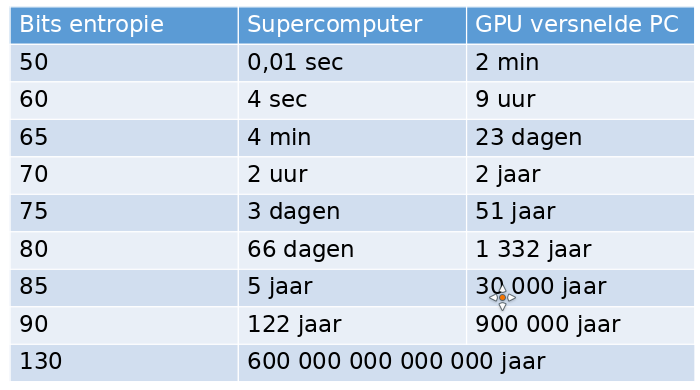
\includegraphics[width=0.5\textwidth]{wachtwoord-entropie.png}
    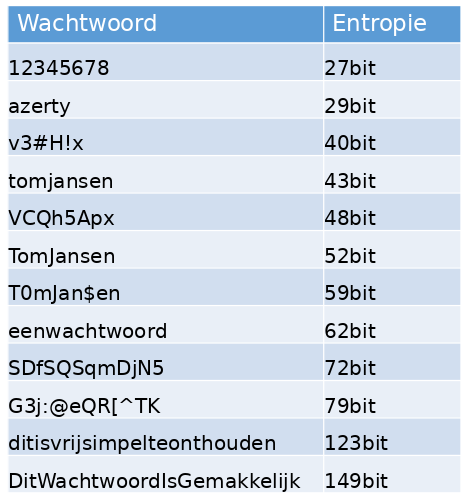
\includegraphics[width=0.3\textwidth]{wachtwoord-entropie2.png}
    \caption{Entropie van een wachtwoord}
\end{figure}

\begin{itemize}
    \item Entropie = uitgedrukt in bits
    \item Beste wachtwoorden zijn vooral voldoende lang
    \item Opgelet voor wachtwoorden in woordenlijsten
    \item Vaak gebruikte wachtwoorden zijn gekend
    \item Enorme lijsten met wachtwoorden zijn beschikbaar
    \item Vaak succesvolle aanval op anders toch complexe wachtwoorden
    \item \url{https://howsecureismypassword.net/}
    \item \url{https://haveibeenpwned.com/}
\end{itemize}

\subsubsection{Tips}

\begin{itemize}
    \item Gebruik geen logisch patroon
    \item Mijd hergebruik voor verschilende diensten (ook niet azertyTwitter en azertyFacebook, etc)
    \item Wijzig je wachtwoorden regelmatig
    \item Leen nooit een wachtwoord uit aan iemand anders
    \item Gebruik waar mogelijk een $\text{2}^{\text{de}}$ factor voor authenticatie (2FA) of multi-factor authenticatie (MFA)
    \item Maak eventueel gebruik van een \underline{wachtwoordkluis}
    \item Let erop door de organisatie goedgekeurde wachtwoordkluis-software te gebruiken
    \item Noteer wachtwoorden NOOIT waar deze door derden kunnen worden achterhaald
\end{itemize}

\subsection{Beveiliging op `Hebben'-basis}

\begin{itemize}
    \item Smartcards
    \item Dongles
    \item Transponder (=soort sleutel)
    \item Digipass (=merk van authenticatiediensten en -producten)
    \item Google Authenticator (=smartphone-app)
\end{itemize}

\subsection{Beveiliging op `Zijn'-basis': biometrische beveiliging}

\begin{itemize}
    \item Iris-scanner
    \item Vingerafdruk
    \item Stem
\end{itemize}

\subsection{Combinatie van meerdere authenticatiemethodes}

\begin{itemize}
    \item 2FA en MFA
    \item Bij voorkeur kiezen tussen methodes op \textit{verschillende} werkingsbasis
\end{itemize}

\subsection{Fysische toegang}

\begin{itemize}
    \item Onvergrendelde schermen
    \item Toegangscontrole serverroom
    \item Hardware aanpassingen of diefstal
    \begin{itemize}
        \item Asset management software
    \end{itemize}
    \item Toegang tot het netwerk
    \item Introductie van vreemde software
    \item Opstarten vanaf andere media
\end{itemize}

\subsection{Privilege escalation}

= zichzelf op een ander gebruikersniveau zetten

\begin{itemize}
    \item Horizontal escalation
    \begin{itemize}
        \item Session hijacking van een andere gebruiker
        \item = toegang verkrijgen van het account van een andere gebruiker
        \item bv: inloggen in Facebook en via je account in het account van een andere gebruiker geraken
    \end{itemize}
    \item Vertical escalation
    \begin{itemize}
        \item = `privilege elevation'
        \item Meer machtigingen verwerven
    \end{itemize}
\end{itemize}


\section{Backup}

\begin{itemize}
    \item Essentieel voor het beschermen van data
    \item Concrete back-up policy
    \item Disaster recovery paln
\end{itemize}

\subsection{Veelgebruikte backup-media}
\begin{itemize}
    \item Tape
    \item Harddisk
    \item USB-stick
    \item Cloud-backup
\end{itemize}

\bold{RAID is geen backup:} beschermt niet tegen meeste risico's. Helpt alleen bij falen van de harddisk. 

\subsection{LTO Tapes}

LTO = Linear Tape Open = open standaard

\begin{itemize}
    \item Worden nog altijd gebruikt, up-to-date
    \item Hoge capaciteit (10-12TB per tape)
    \item Hoge transfer rate (500MB/s)
    \item Redeljk goedkoop, iets duurder dan harde schijven per GB
\end{itemize}

\subsubsection{LTO Drive}


\begin{itemize}
    \item Toestel om LTO Tapes te lezen/schrijven
    \item Heel duur (duizenden euros)
\end{itemize}

\begin{figure}[H]
    \centering
    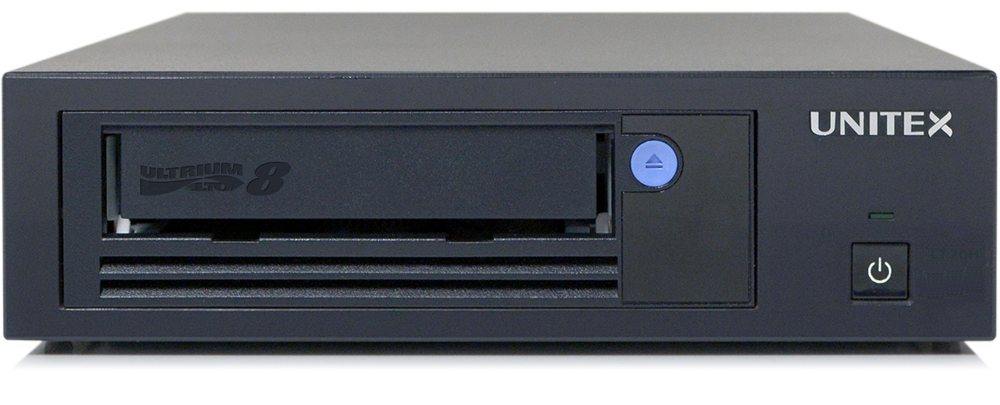
\includegraphics[width=0.2\textwidth]{lto-drive-single.png}
    \caption{LTO drive voor 1 tape}
\end{figure}

\begin{figure}[H]
    \centering
    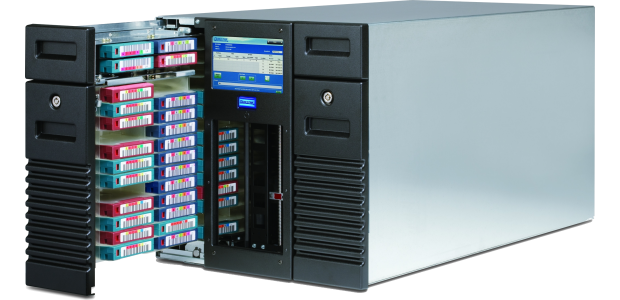
\includegraphics[width=0.3\textwidth]{lto-drive-multi.png}
    \caption{LTO tape robot: 12000-15000 euro}
\end{figure}


\subsection{Eigenschappen van een correcte backup}

\begin{itemize}
    \item Offline
    \item Beveiling tegen aanpassing (Integrity)
    \item Beschikbaar (Availability)
    \item Veilig opgeslegen (Confidentiality)
    \item Betrouwbaar 
\end{itemize}

\subsection{3-2-1 regel}

\begin{figure}[H]
    \centering
    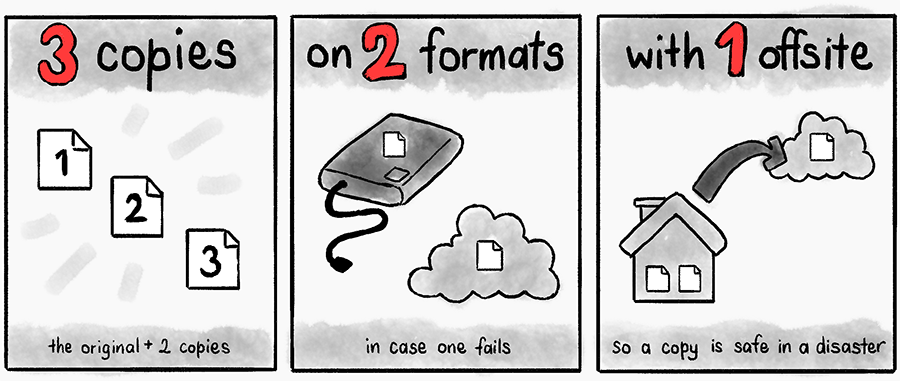
\includegraphics[width=0.3\textwidth]{321-regel.png}
    \caption{3-2-1-regel: 3 copies, 2 formats, 1 offsite}
\end{figure}


\subsection{Cloud back-up}

\begin{itemize}
    \item Wat met aansprakelijkheid?
    \begin{itemize}
        \item Je hebt geen controle over het systeem
    \end{itemize}
    \item Wat met beschikbaarheid?
    \begin{itemize}
        \item Niet zo makkelijk om de hele backup te downloaden uit de cloud (bandbreedtelimieten, snelheid, \dots)
    \end{itemize}
    \item Wat met vertrouwelijkheid?
    \begin{itemize}
        \item Wie heeft allemaal toegang tot de data?
    \end{itemize}
    \item Wetgeving?
    \item Wel zeer eenvoudig en gemakkelijk
\end{itemize}

\subsection{Back-up policy}

\begin{itemize}
    \item Hoge back-up frequentie
    \item Goede back-up strategie
    \item Type back-up
    \item Opslag van back-up:
    \begin{itemize}
        \item Dicht bij de server voor snelle toegang
        \item Op een andere locatie voor veiligheid
    \end{itemize}
    \item Controle van integriteit back-up
    \item Testen van disaster-recovery plan
\end{itemize}

\subsubsection{Grootvader - vader - zoon-systeem}

\textcolor{red}{\bold{WORDT GEVRAAGD OP EXAMEN}}

\begin{figure}[H]
    \centering
    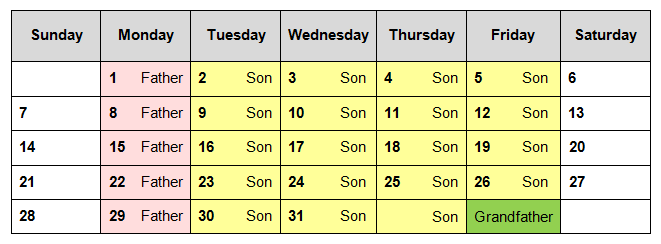
\includegraphics[width=0.5\textwidth]{gfs.png}
    \caption{Grootvader-vader-zoon systeem}
\end{figure}

\bold{Bv:} Elke maandag een backup op de `Father'-schijf, elke andere weekdag een backup op de `Zoon'-schijf, elke maand een backup op de `Grootvader'-schijf.

\begin{itemize}
    \item Back-uprotatie:
    \begin{itemize}
        \item Meerdere backups, waarbij de oudste backup wordt overschreden bij het maken van een nieuwe backup.
        \item Zo heb je altijd een chronologische opeenvolging van backups
    \end{itemize}
    \item Archivering
    \item Backup moet zowel:
    \begin{itemize}
        \item Actueel zijn
        \item Voldoende teruggaan in de tijd
    \end{itemize}
\end{itemize}

\url{https://en.wikipedia.org/wiki/Backup_rotation_scheme#Grandfather-father-son}

\subsection{Belangrijk}

\begin{itemize}
    \item CIA-model over de hele lijn
    \item Moet worden getest
    \item Moet effectief worden uitgevoerd
\end{itemize}

\section{Penetration testing}

= testen van security

\begin{itemize}
    \item Wat gebeurt er \textit{echt}?
    \item Wat kan de hacker doen?
    \item $\Rightarrow$ bewustwording van security
    \item Wettelijke beperkingen: toestemming nodig van eigenaar!
\end{itemize}

\subsection{Black-box testing vs white-box testing}

\subsubsection{Black-box testing}

\begin{itemize}
    \item Binnenbreken zonder dat je iets weet over het target
    \item Iets van waarde proberen uit het systeem te halen
    \item Je weet niet wat/waar je moet aanvallen
    \item Minder efficient
\end{itemize}

\subsubsection{White-box testing}

\begin{itemize}
    \item Gaan kijken naar de serverruimte, rondleiding krijgen van eigenaar
    \item Documentatie doorlezen
    \item Volledige toegang tot infrastructuur, om te kijken wat er beter kan
    \item Consulting, raad vragen
    \item Demonstratieve luik is helemaal weg: moeilijker om te tonen aan de eigenaar wat een hacker zou kunnen doen.
    \item Veel efficienter
\end{itemize}

\subsection{Fase 1: Reconnaissance}

Reconnaissance = Information gathering = OSINT

\begin{itemize}
    \item Verzamelen van informatie over het target
    \begin{itemize}
        \item Algemene info
        \item Bedrijfsinfo
        \item E-mailadressen
        \item Organigram (=hi"erarchie van het bedrijf)
        \item Leveranciers
        \item \dots
    \end{itemize}
    \item Inzetbaar voor social engineering
    \item Spear-phishing
\end{itemize}

\subsubsection{Tools \& attack surfaces}

\begin{itemize}
    \item Google!
    \item DNS
    \item Sociale netwerken
    \item Bedrijfssite
    \item \dots
\end{itemize}

\subsection{Fase 2: Netwerk scanning}

\begin{itemize}
    \item nmap : overlopen van services op het systeem
    \item port-scanners
    \item SNMP
    \item Wireshark / sniffing
    \item \dots
\end{itemize}

\subsubsection{Network reconnaissance}

\begin{itemize}
    \item Sniffing
    \item Port scanning
    \item OS fingerprinting
    \item Detectie van gebruikte software
    \item DNS zone data
    \item Information harvesting
\end{itemize}

\subsection{Fase 3: Vulnerability assessment}

\begin{itemize}
    \item Vulnerabilty scanners, zoals: Nexpose, Retina/Iris
    \begin{itemize}
        \item Geeft een rapport van kwetsbaarheden op het systeem
        \item Niet context-bewust: een scanner weet niet per se welke bestanden intressant zijn
        \item Heel veel informatie
    \end{itemize}
    \item Identificatie uit CVE (common vulnerabilities and exposures) database
\end{itemize}

\subsection{Fase 4: Exploit, Access, penetratie}

\begin{itemize}
    \item De gevonden kwetsbaarheden uitbuiten (exploiten)
    \item Toegang verkrijgen tot het systeem
    \item Opgelet naar beschikbaarheid/vertrouwelijkheid/legaliteit
\end{itemize}


\subsection{Fase 5: Maintaining access}

\begin{itemize}
    \item Het behouden van de verkregen toegang
    \item Covering tracks: sporen proberen uit te wissen
    \item Proberen zo veel mogelijk in-memory te doen: geen permanente wijzigingen aanbrengen aan het systeem.  
    \item Opgelet naar beschikbaarheid/vertrouwelijkheid/legaliteit
\end{itemize}

\section{Sociale media}

\begin{itemize}
    \item Oversharing: alles in detail delen met iedereen
    \item Mensen hebben niet door wat de impact daarvan is
    \item \url{https://www.youtube.com/watch?v=F7pYHN9iC9I}
    \item Op sociale media posten = vertellen aan willekeurige vreemden
    \item Deel nooit een foto van je bankkaart op sociale media
\end{itemize}

\subsection{Metadata}

= data over data

\bold{Voorbeeld:} als je een foto trekt wordt daar veel metadata over opgeslagen (=EXIF-data)

\begin{itemize}
    \item Plaats en GPS-locatie
    \item Exacte tijd/datum
    \item Cameramerk en type
    \item \dots
\end{itemize}

Dit is mogelijks bruikbare informatie bij aanvallen. 
Het kan ook soms een \bold{informatielek} zijn voor de organisatie waarvoor je werkt.

\section{Social engineering}

\begin{itemize}
    \item Zie Kevin Mitnick's "The art of deception"
    \item De menselijke schakel in security
    \item Misbruik van inherente psychologische kenmerken van mensen
    \item Vertrouwen, hulpvaardigheid, empathie, \dots misbruiken
\end{itemize}

\subsection{Pretexting}

= Het cre"eeren van een scenario om het 
slachtoffer te engageren zodat het slachtoffer 
makkelijker informatie weggeeft of acties onderneemt 
die het slachtoffer normaal niet zou doen.


\subsubsection{Hoe?}

\begin{itemize}
    \item Vertrouwen verkrijgen in uniform, met een impersonatie, \dots
    \item Over telefoon, gebruik van interne lijn, \dots
    \item Over email, spoofing, \dots
\end{itemize}

\subsection{Informatielekken}

\begin{itemize}
    \item Afval met gevoelige inhoud vernietigen (tegengaan van dumpsterdiving)
    \item Voorzichtig omgaan met vertrouwelijke info
    \item Geen kritische info op toestellen of prikborden
    \item In een bedrijf geraken via de nooduitgang door bvb te praten met de rokers en dan samen naar binnen te wandelen, terwijl je doet alsof je daar werkt.
\end{itemize}

\subsubsection{Remediering}

\begin{itemize}
    \item Opleiding
    \item Waakzaamheid
    \item Strike security policy
\end{itemize}

\subsection{Afluisteren}

\begin{itemize}
    \item Op het draadloos netwerk
    \item Op de kabel
    \item Sniffing (=de diefstal/interceptie van data via het onderscheppen van netwerkverkeer)
    \item Hubs vs Switches: sniffing op een hub is veel eenvoudiger, worden ook minder gebruikt
\end{itemize}



\subsubsection{Man in the middle attack}

\begin{itemize}
    \item WiFi MITM (bvb met openbare hotspots)
    \item Evil-twin access point: 
    \begin{itemize}
        \item = Een access point die je zelf controleert met dezelfde SSID als een ander access point in de omgeving
        \item Mensen connecteren op uw access point $\Rightarrow$ je ziet hun inloggegevens 
        \item Je kan uw access point verbinden met internet, zodat die mensen inloggen op Facebook, Email $\Rightarrow$ die inloggegevens kan je dan ook onderscheppen
    \end{itemize} 
    \item Vrij simpel implementeerbaar
    \item Bv: met een WiFi Pineapple
\end{itemize}

\begin{figure}[H]
    \centering
    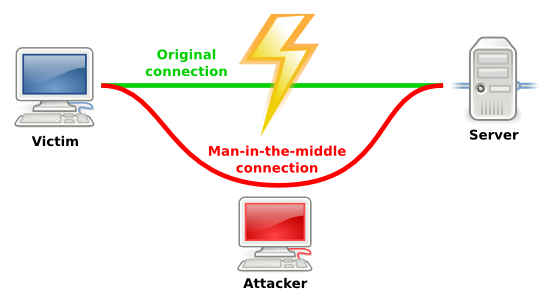
\includegraphics[width=0.5\textwidth]{mitm-attack.png}
    \caption{Man in the middle attack}
\end{figure}

\subsubsection{Remediering}
\begin{itemize}
    \item Intelligente switches met port-shutdown
    \item Encryptie: versleuteld internetverkeer (geen FTP, HTTP, Telnet, \dots. Beter: SFTP, HTTPS, SSH)
\end{itemize}

\section{Wireless}

\begin{itemize}
    \item WiFi
    \begin{itemize}
        \item Vrijwel overal aanwezig
        \item Laptop, tablet, \dots
        \item Maar stopt niet aan de eigendomsgrens 
    \end{itemize}
    \item NFC
    \item Bluetooth
    \item Wireless keyboards, muizen, \dots
\end{itemize}

\subsection{Vreemde netwerken}

\begin{itemize}
    \item Openbaren netwerken kunnen worden afgeluisterd
    \item Verkeer op niet-vertrouwde netwerken kan worden afgeluisterd
    \item WEP-beveiliging is redelijk onveilig
\end{itemize}

\begin{figure}[H]
    \centering
    \includegraphics[width=0.5\textwidth]{vreemde-netwerken.png}
    \caption{Vreemd netwerk m.b.v. een rogue wireless access point}
\end{figure}

\subsection{Frequentie}

\begin{itemize}
    \item Twee kampen: 2.4GHz (en 5GHz) vs SubGHz
    \item Alles dat hogere bandbreedte nodig heeft $\Rightarrow$ 2.4 en 5GHz
    \item Alles dat niet zo veel bandbreedte nodig heeft $\Rightarrow$ SubGHz
\end{itemize}


\begin{figure}[H]
    \centering
    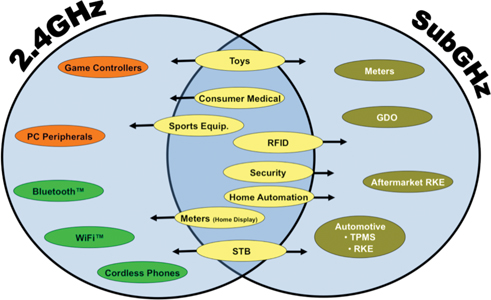
\includegraphics[width=0.5\textwidth]{2.4-subghz.png}
    \caption{2.4GHz/5GHz vs SubGHz}
\end{figure}


\section{Virussen en malware}

\subsection{Virussen}

\begin{itemize}
    \item Bestandsvirussen (.exe en .com)
    \item Bootsectorvirussen
    \item Macrovirussen
    \item Wormen = virus zonder symbiant (=drager)
    \item Virustechnologie
\end{itemize}

\subsubsection{Virustechnologie}

\begin{itemize}
    \item Polymorphisme
    \begin{itemize}
        \item = het virus gaat zichzelf gaan wijzigen
    \end{itemize}
    \item Hybride
    \begin{itemize}
        \item = virus met meer dan 1 infectiemethode
    \end{itemize}
    \item Multipart
    \begin{itemize}
        \item = virus dat uit meerdere delen bestaat, modulair
    \end{itemize}
    \item Stealth
    \begin{itemize}
        \item = virus dat zichzelf gaat verbergen
    \end{itemize}
    \item Droppers
    \begin{itemize}
        \item = software dat virulente code gaat inbrengen (droppen) in het systeem om daar achter te laten
    \end{itemize}
\end{itemize}

\subsection{Malware}

\begin{itemize}
    \item Trojans
    \begin{itemize}
        \item Software die adverteert iets goed te doen, maar slechte bedoelingen heeft
    \end{itemize}
    \item Spyware
    \begin{itemize}
        \item Probeert zoveel mogelijk informatie te vergaren
    \end{itemize}
    \item Adware
    \begin{itemize}
        \item Toont advertenties aan de gebruiker
    \end{itemize}
    \item Scareware
    \begin{itemize}
        \item Software met als doel je bang te maken
    \end{itemize}
    \item RATs = Remote Access Tools:
    \begin{itemize}
        \item Bv: backorifice $\Rightarrow$ neemt het systeem over
    \end{itemize}
    \item Ransomware
\end{itemize}


\subsection{Hardware}
\begin{itemize}
    \item Hardware backdoor in toestellen
    \item Rubber ducky
    \item BadUSB = USB-stick die zichzelf oplaad om dan een stroomstoot te geven aan de computer. Kan de USB-bus kapot maken of zelf het hele moederbord
\end{itemize}


\subsubsection{BIOS}

BIOS = Basic Input/Output System 

= firmware die onder andere het besturingssyteem van een PC opstart

\begin{itemize}
    \item Chernobyl virus $\Rightarrow$ $\text{1}^{\text{ste}}$ virus die BIOS wist
\end{itemize}

\subsubsection{UEFI}

= Unified Extensible Firmware Interface, vervangt tegenwoordig de BIOS op computers):

\begin{itemize}
    \item Is universeel en uitbreidbaar
    \item UEFI "Bootkit" voor Windows 8 
    \begin{itemize}
        \item Bootkit = rootkit die voor het operating system wordt geladen, tijdens de UEFI
        \item Kan full disk encryption systemen ontgrendelen
    \end{itemize}
    \item Rakshasa = hardware backdoor, praktische aanval theoretisch mogelijk
\end{itemize}

\subsection{Misleidende informatie}

\begin{itemize}
    \item Manipulatie van informatie
    \item Messagebox: welke info wordt bepaalt door wie?
    \item URL's: welke URL zit werkelijk achter een link?
    \begin{itemize}
        \item <a href="site.evil-haxsor.whatever">www.disney.com</a>
    \end{itemize}
\end{itemize}

\begin{figure}[H]
    \centering
    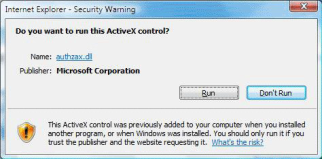
\includegraphics[width=0.3\textwidth]{messagebox.png}
    \caption{Messagebox}
\end{figure}

\subsubsection{Kwaadaardige links}

\begin{itemize}
    \item Link kan een ander doel hebben dan wordt weergegeven
    \item Opgepast voor homograaf-URL (punycode)
    \begin{itemize}
        \item Bvb Cyrilische tekens in een URL:
        \item 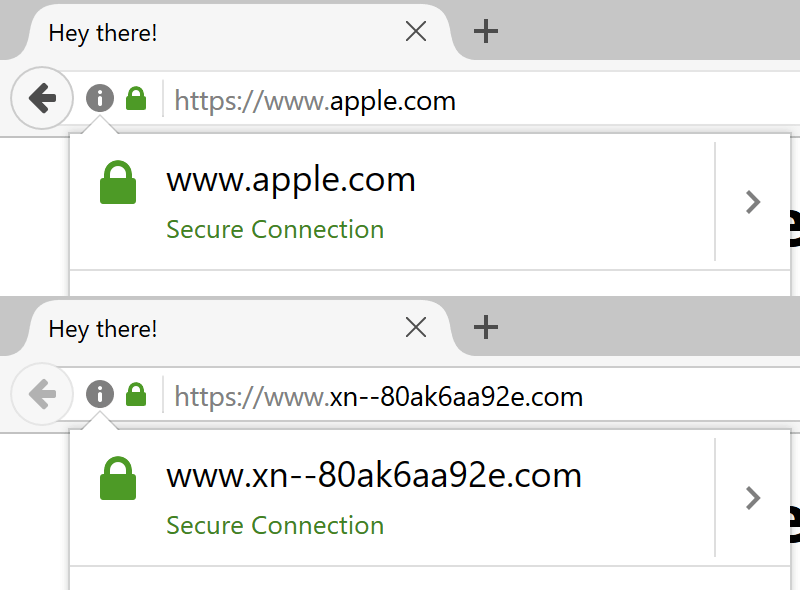
\includegraphics[width=0.2\textwidth]{link2.png}
    \end{itemize}
    \item Controleer de link! 
    \begin{itemize}
        \item 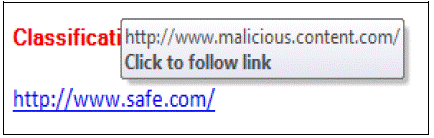
\includegraphics[width=0.3\textwidth]{link.png}
    \end{itemize}
    \item 'Open folder to view files' kan eigenlijk een link zijn naar een .exe als de maker van de software het zo noemt
    \begin{itemize}
        \item 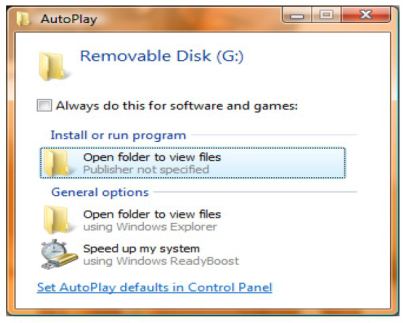
\includegraphics[width=0.3\textwidth]{open-folder.png}
    \end{itemize}
\end{itemize}

\section{Cloud en Software As A Service (SaaS)}

\begin{itemize}
    \item Er bestaat een onderscheid tussen Personal / Private / Public Cloud
    \begin{itemize}
        \item Personal = servers in eigen huis
        \item Private = Iemand anders zijn systemen, eigen privéruimte
        \item Public = Iemand anders zijn systemen, gedeelde ruimte
    \end{itemize}
    \item Afhankelijk van aanbieder van de "hosted service"
    \item CIA analyse blijft relevant in de cloud, enkele potentiele problemen: 
    \begin{itemize}
        \item Confidentialiteit: PRISM (=afluistersysteem van de Amerikaanse afluisterdienst NSA)
        \item Integriteit: Malware / Synolocker (=ransomware voor Synology NAS-systemen) / \dots
        \item Beschikbaarheid: Internet Carriers / overheden
    \end{itemize}
\end{itemize}

\subsection{Cloud diensten}

\begin{itemize}
    \item Kan zeer handig zijn
    \item Een extra dienst is een extra risico
    \item Meerdere clouddiensten = de informatie staat op meerdere plaatsen
    \item De organisatie kan zelf niet weten waar alle informatie is opgeslagen
    \item Gebruik enkel de door de organisatie aanbevolen en goedgekeurde clouddiensten
\end{itemize}

\begin{figure}[H]
    \centering
    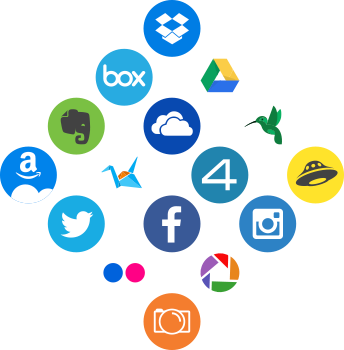
\includegraphics[width=0.2\textwidth]{cloud-diensten.png}
    \caption{}
\end{figure}


\subsection{Acceptabel gebruik / Policy}

\begin{itemize}
    \item Geeft vaak de indruk de gebruiker van te willen beperken
    \item Porbeert een balans te vinden tussen acceptabel risico en bruikbaarheid
    \item Is noodzakelijk om de systemen beheersbaar te houden
    \item Dient steeds strikt te worden opgevolgd
\end{itemize}

\subsection{Migratie naar cloud diensten}

\begin{itemize}
    \item E-mail / groupware oplossingen
    \item Allicht veiliger dan een eigen exchange-server
    \item On-line boekhoudsoftware
    \item Onfeilbaar? Perfect? 
    \item Threat model / risk analysis: analyse van meest kwetsbare onderdelen
    \item Zijn er andere threats dan bij een lokale server?
\end{itemize}

\subsubsection{Voordelen / Unique Selling Point (USP)}

\begin{itemize}
    \item Toegang van overal
    \item Samenwerken met derden
    \item Automatische back-up
\end{itemize}

\subsubsection{Nadelen}

\begin{itemize}
    \item Vendor lock-in: het is vaak omslachtig om van de ene naar de andere clouddienst over te stappen
    \item Vertrouwelijkheid: kan je de service wel vertrouwen?
    \item Prijs?
    \item Continu"iteit?
\end{itemize}

\section{Bring Your Own Device (BYOD)}

= mensen gebruiken hun persoonlijke apparaten op het werk / om te werken.

\subsection{Problemen}

\begin{itemize}
    \item Potentieel gebruik door derden in thuisomgeving
    \item Diverse apps worden binnengebracht (malware)
    \item Compatibiliteitsproblemen
    \begin{itemize}
        \item Sommigen gebruiken Windows, sommigen macOS, sommigen Linux.
    \end{itemize}
    \item Problemen met ondersteuning
    \begin{itemize}
        \item De IT-dienst moet een hele groep apparaten ondersteunen in plaats van enkel degene die ze geven aan werknemers.
    \end{itemize}
\end{itemize}

\subsection{Mobiele apparaten}

Mobiele apparaten bevatten heel veel gevoelige info en zijn daarom een groot doelwit:

\begin{itemize}
    \item Bevatten enorme hoeveelheid vertrouwelijke gegevens
    \item Wordt ook vaak gebruikt als 2de factor bij authenticatie
    \item Wordt vaak gebruikt om wachtwoorden terug te stellen
    \item Niet alle apps zijn te vertrouwen
    \item Een app kan info naar de ontwikkelaar doorsturen (privacysettings)
    \item Vergrendel je smartphone altijd
    \item Gebruik geen telefoon met gevoelige gegevens voor spelletjes
    \item Opgepast voor misleidende meldingen en advertenties
    \item Laat je smartphone niet door derden gebruiken (bijv. door kinderen)
\end{itemize}

\subsubsection{Mobile malware}

\begin{figure}[H]
    \centering
    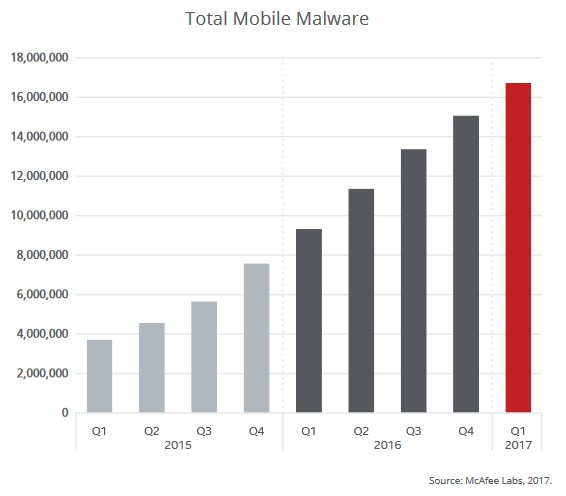
\includegraphics[width=0.5\textwidth]{mobile-malware.jpg}
    \caption{Mobile malware door de jaren heen}
\end{figure}

\begin{figure}[H]
    \centering
    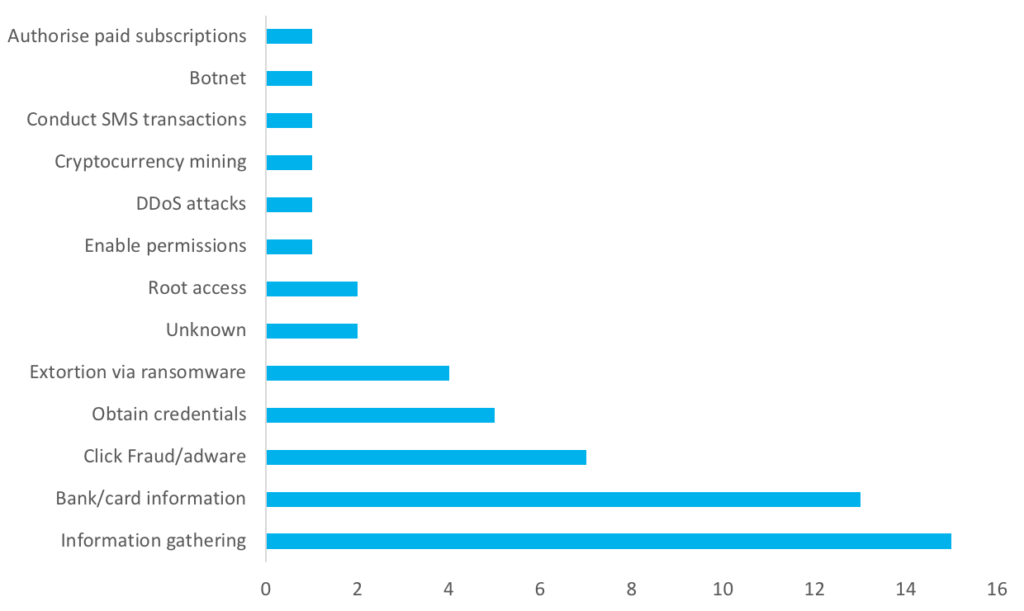
\includegraphics[width=0.5\textwidth]{mobile-malware-types.png}
    \caption{Voornaamste types exploits op Android}
\end{figure}

\begin{itemize}
    \item De meeste problemen op Android
    \item De ergste problemen op iPhone
    \begin{itemize}
        \item MDM (Mobile Device Management)
        \item = software om een toestel te beheren, configureren, \dots
        \item = Volledige remote controle, apps/malware op afstand installeren
        \item Fake MDM software bestaat op iPhone, minder op Android
    \end{itemize}
    \item Oplossing: MDM software zoals Samsung Knox
\end{itemize}

\begin{figure}[H]
    \centering
    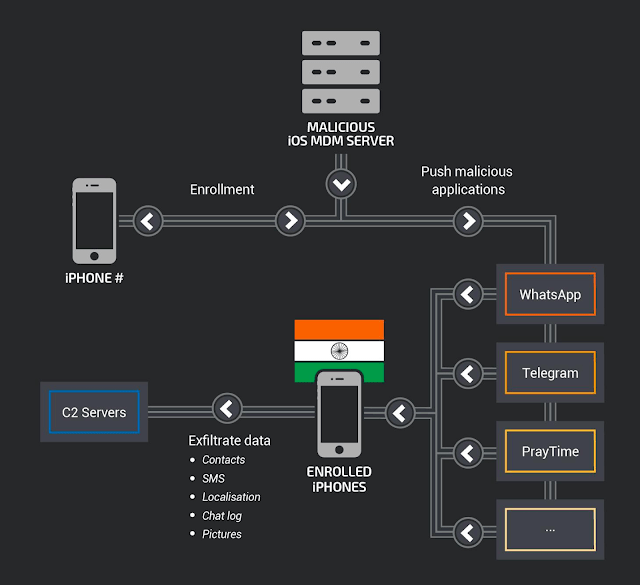
\includegraphics[width=0.5\textwidth]{malware-iphone.png}
    \caption{}
\end{figure}

\section{Beschikbaarheid}

\subsection{High Availability}

\begin{itemize}
    \item = (bijna) altijd beschikbaar
    \item High availability op netwerkniveau
    \item High availability systemen (=always on devices)
    \item Clusters / load balancing (= meerdere high available servers die eenzelfde dienst kunnen aanbieden)
    \item Redundante servers
    \item Redundante serverruimte (disaster center, volledige verdubbeling van een datacenter)
    \item Virtualisatie: 
    \begin{itemize}
        \item deel van infrastrucuur abstraheren
        \item Problemen oplossen in VMs
    \end{itemize} 
\end{itemize}

\subsection{Externe netwerk bedreigingen}

\begin{itemize}
    \item (Distributed) Denial of Service: (D)DOS
    \item Portscanning
    \item Sniffers
    \item Man in the Middle (MITM)
    \item Spoofing
    \item \dots
\end{itemize}

\subsubsection{Denial of Service (DoS)}
\begin{itemize}
    \item E-mail bommen: vloedgolf van vele en/of grote e-mails, om de computer of mail service lam te leggen
    \item Logic bomb: een soort tijdbom. De code wordt geactiveerd waneer een bepaalde actie gebeurt
    \item Repetitive login
    \item SYN-Flooding
    \begin{itemize}
        \item Misbruik maken van het TCP/IP protocol
        \item Constant SYN-pakketten sturen met foute bron-IP-adressen
        \item De server krijgt geen ACK omdat hij de SYN-ACK stuurt naar het verkeerde IP-adres.
    \end{itemize}
\begin{figure}[H]
    \centering
    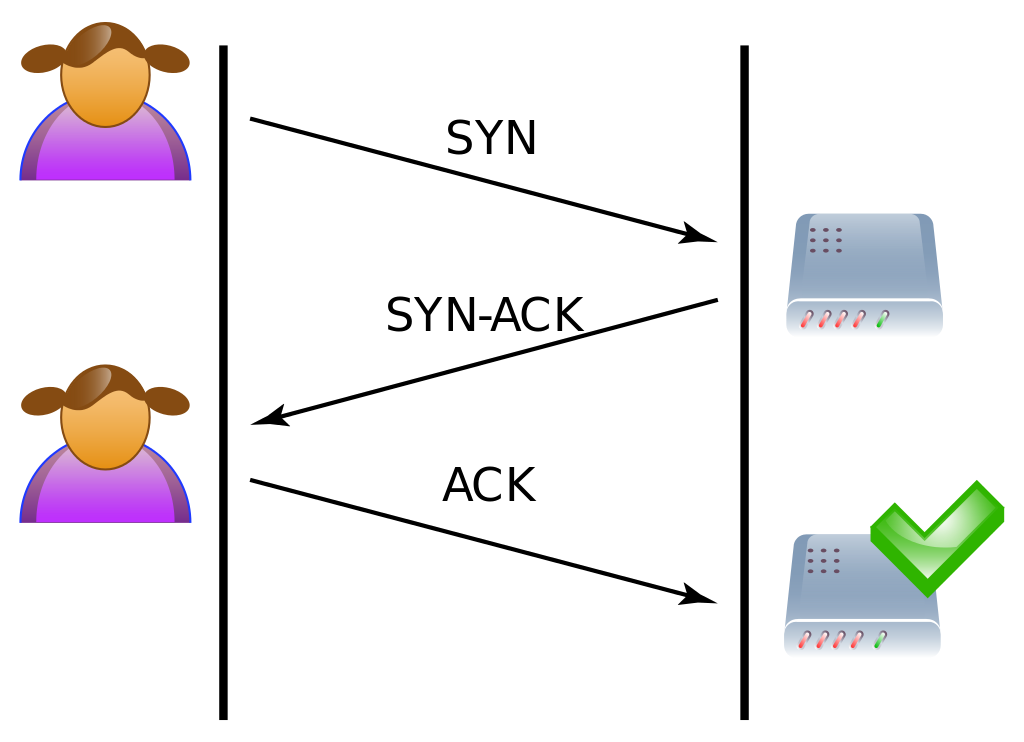
\includegraphics[width=0.3\textwidth]{tcp-normal.png}
    \caption{Normal TCP/IP three-way handshake}
\end{figure}

\begin{figure}[H]
    \centering
    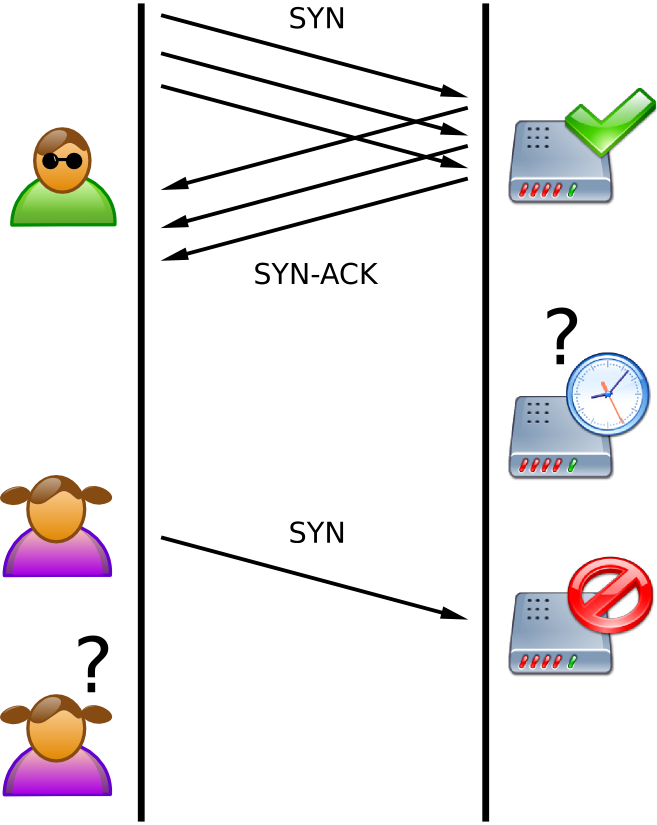
\includegraphics[width=0.3\textwidth]{tcp-synflood.png}
    \caption{SYN Flooding}
\end{figure}
    \item UDP-Flooding
    \begin{itemize}
        \item Misbruik maken van het UDP protocol
        \item Een groot aantal UDP pakketten sturen naar willekeurige poorten van een target
        \item Het target zal:
        \begin{enumerate}
            \item Kijken of een applicatie luistert naar die poort
            \item Vaststellen dat geen applicatie luistert naar die poort
            \item Antwoorden met een ICMP Destination Unreachable pakket
        \end{enumerate}
        \item Het target zal constant hiermee bezig zijn $\Rightarrow$ kan geen service aanbieden aan echte clients
    \end{itemize}
    \item Ping of death
    \begin{itemize}
        \item Een normale ping is minder dan 100 bytes groot
        \item Het is mogelijk om pings van een andere grootte (max. 65535 bytes) te sturen
        \item Op oudere systemen: buffer overflow mogelijk $\Rightarrow$ system crash
        \item Tegenwoordig: Ping Flooding: overbelasting $\Rightarrow$ minder toegankelijkheid van normaal internetverkeerd
    \end{itemize}
\end{itemize}




\subsubsection{Distributed DoS (DDOS)}

\begin{itemize}
    \item DoS simultaan uit verschillende locaties
    \item Zeer moeilijk tegen te houden
    \item Meestal zijn de drones geinfecteerde thuis-PCs
\end{itemize}

\begin{figure}[H]
    \centering
    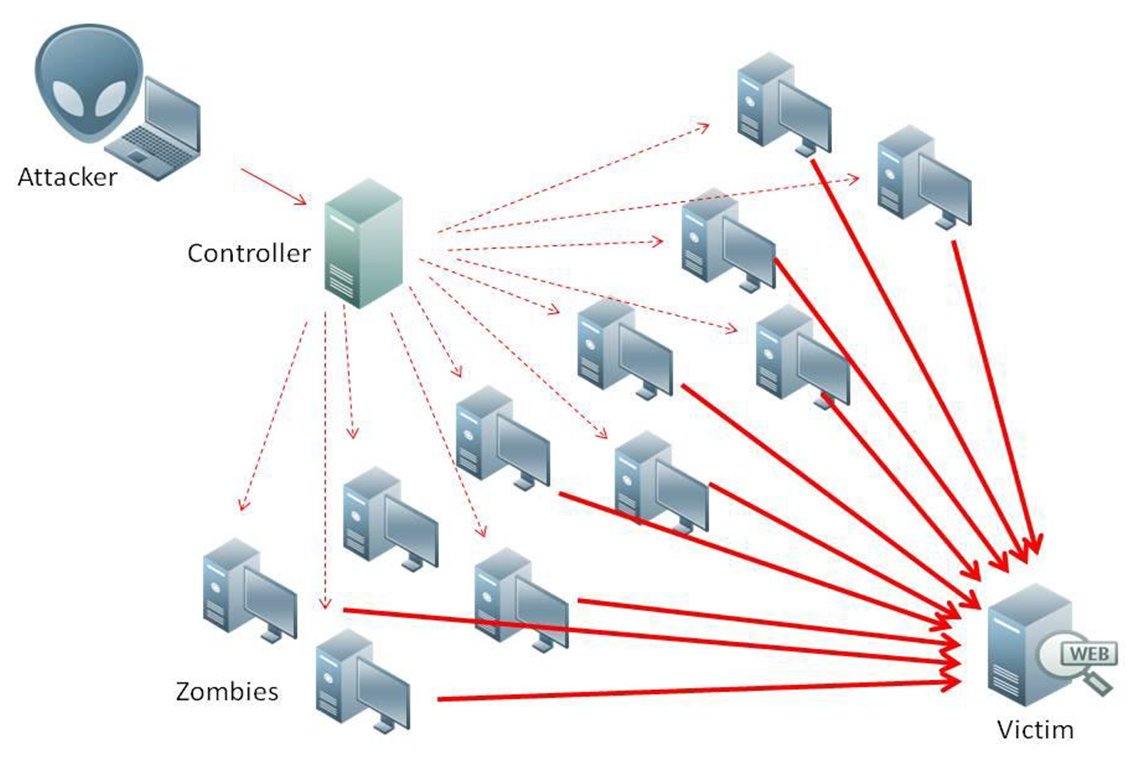
\includegraphics[width=0.5\textwidth]{ddos.png}
    \caption{DDoS}
\end{figure}

\bold{Hoe een DDoS tegenhouden?}

\begin{itemize}
    \item Capaciteit uitbreiden (maar dit is zelden economisch intressant)
    \item DDoS-beveiliging \& caching dienst zoals CloudFlare DDoS Protection
    \begin{itemize}
        \item Caching
        \item Grote server-redundantie over de hele wereld
        \item Keerzijde: CloudFlare is eigenlijk een Man In The Middle attack: CloudFlare zit altijd tussen client en server $\Rightarrow$ alle verkeer leesbaar door CloudFlare
    \end{itemize}
\end{itemize}

\subsubsection{Spoofing}

= Het vervalsen van informatie in de header:

\begin{itemize}
    \item IP spoofing
    \item MAC spoofing
    \item Email spoofing
    \item \dots
\end{itemize}

\subsection{Uptime}

Uptime != Availability

\begin{itemize}
    \item 99.9\% available = 8.76 uur per jaar onbeschikbaar
    \item 99.999\% available = 5.26 min per jaar onbeschikbaar
    \item Wordt vaak genoteerd als `3 nines' (=99.9\%), `5 nines' (=99.999\%)
    \item Als je voor `5 nines' availability betaalt, vertaalt dit niet noodzakelijk naar uptime:
    \begin{itemize}
        \item Stel: je hebt een webshop die meerdere services nodig heeft (website, backend, database, \dots)
        \item Elke service heeft `5 nines' availability
        \item Als 1 van de services down is, stopt de hele webshop met werken (=downtime)
        \item $\Rightarrow$ het kan dus zijn dat de uptime kleiner is dan de 99.999\% waarvoor je betaald hebt
    \end{itemize}

\end{itemize}

\section{Web security}

\begin{itemize}
    \item Een belangrijke attack surface / point of entry (PoE)
    \item Belangrijk naar reputatie
    \item CMS-Systemen  (wordpress, drupal, joomla, ..)
    \item Authenticatie / escalation
    \item OWASP: \url{https://www.owasp.org}
\end{itemize}

\subsection{Vaak voorkomende problemen}

\begin{itemize}
    \item Injection (bvb SQL injection, command injection, \dots)
    \item Cross site scripting (XSS)
    \item Cookie stealing
    \item Zie OWASP Top 10: top 10 meest voorkomende technieken
\end{itemize}

\subsection{Security scanners}

Tools om websites te scannen op gekende kwetsbaarheden:

\begin{itemize}
    \item Nessus
    \item Nikto
    \item OpenVAS
    \item OWASP Mantra
    \item Burpsuite
\end{itemize}

\subsection{Risico's}

\begin{itemize}
    \item "Defacement"
    \item Lek van credentials
    \item Reputatie van het bedrijf
    \item Diefstal (bij bvb webshops)
    \item Totale controle van server \& alle systemen
    \item \dots
\end{itemize}

\subsection{Remediation}

\begin{itemize}
    \item Don't be stupid
    \item Gebruik sanitation libraries (no DIY!)
    \item Update site framework, plugins \& libraries
    \item Prepared statements for SQL (to remediate SQL injection)
    \item Authentiation frameworks
\end{itemize}

\section{Gegevensbescherming}

\subsection{CIA-model}

\begin{itemize}
    \item Confidentiality: Gegevens confidentieel houden: beschermen tegen derden
    \item Integrity: Waken over integriteit van gegevens: beschermen tegen ongeoorloofde aanpassingen
    \item Availability: Gegevens beschikbaar houden: beschermen tegen verlies
\end{itemize}

\subsection{GDPR}

= General Data Protection Regulation

\begin{itemize}
    \item AVG = Algemene Verordering Gegevensbescherming
    \item Persoonsgegevens = alle gegevens die kunnen gebruikt worden om iemand te identificeren.
    \item Anonimiseren of pseudonimiseren van gegevens is mogelijk
    \begin{itemize}
        \item Geanonimiseerde gegevens = gegevens waarvan geen persoonsgegevens kunnen worden achterhaald
        \item Gepseudonimiseerde gegevens = gegevens waarvan persoonsgegevens alleen kunnen worden achterhaald als de gegevens naast de persoonsgegevens worden gelegd.
    \end{itemize}
    \item Goedkeuring voor verwerking is noodzakelijk
    \item Er moet een reden zijn om gegevens te verwerken of op te slaan
\end{itemize}


\subsection{Tips}

\begin{itemize}
    \item Let op met afdrukken
    \item Clean desk policy: laat geen (gevoelige) informatie zomaar op je bureau liggen
    \item Sla gegevens centraal op
    \item Sla gegevens enkel op in door de organisatie goedgekeurde locaties en media
    \item Laat absoluut geen gegevensdragers (USBs, HDDs, \dots) rondslingeren
    \item Vernietig gegevens die niet langer bijgehouden moeten worden
    \item Vernietig gegevens volgens de voorschriften van de organisatie
\end{itemize}

\subsection{Acceptable Use Policy (AUP)}

= Acceptabel gebruik van gegevens

\begin{itemize}
    \item Geeft vaak de indruk de gebruiker te willen beperken
    \item Probeert een balans te vinden tussen acceptabel risico en bruikbaarheid
    \item Is noodzakelijk om de systemen beheersbaar te houden
    \item Dient steeds strikt te worden opgevolgd!
\end{itemize}

\subsection{Buiten het kantoor}

\begin{itemize}
    \item Let op met openbare netwerken: houd u steeds aan de voorschriften / policy (VPN)
    \item Deel nooit interne informatie met derden
    \item Wees waakzaam over wie er kan meeluisteren (kan gebruikt worden bij social engineering)
    \item Opgepast voor diefstal, gegevens kunnen mogelijks worden uitgelezen van een toestel zelfs indien dit beveiligd was
    \item Opgepast met aansluiten van of op externe apparatuur (USBs, netwerkkabels, projector)
\end{itemize}

\subsection{Bedreigingen van binnenin}

\begin{itemize}
    \item Grootste aandeel van veligheidsproblemen wordt veroorzaakt door een actie van binnenin
    \item Spring zorgvuldig om met gepriviligeerde informatie
    \item Vaak worden documenten onbewust doorgestuurd
    \item Wees alert op mogelijke beinvloeding
\end{itemize}

\subsection{Fysieke beveiliging}

\begin{itemize}
    \item Probeer diefstal te voorkomen
    \begin{itemize}
        \item Gebruikmaken van gepaste beveiliging
        \item Bewaar `intressante' spullen uit het zicht
    \end{itemize}
    \item Houd de werkplaats opgeruimd zodat geen confidentiele informatie zichtbaar is
    \item Wees indachtig waar print-outs en documenten liggen. Scherm deze af voor onbevoegden
    \item Meld steeds verdachte activiteiten aan een bevoegd persoon
\end{itemize}

\subsection{Afdwingen}

\begin{itemize}
    \item Afdwingen van de AUP
    \item Door de gebruikers te informeren
    \item De noodzakelijkheid te duiden
    \item Awareness cree"eren bij de gebruikers
\end{itemize}

\subsection{Gedragscode voor de informatiebeheerder}

\begin{itemize}
    \item Voorbeeld ADM gedragscode
    \item Wat mag een beheerder doen?
    \item Waar stopt de privacy van een gebruiker?
    \item $\Rightarrow$ CAO 81 (=Collectieve arbeidsovereenkomst nr 81)
    \begin{itemize}
        \item = Bescherming van de persoonlijke gegevens van werknemers t.o.v. de controle op online-communicatiegegevens
        \item Meer info op leho bij Modules (cao-81.pdf)
    \end{itemize}
\end{itemize}

\section{Risico's}

\begin{itemize}
    \item De mate van bedreiging is niet beheersbaar
    \item De kwetsbaarheid is te reduceren door de implementatie van tegenmaatregelen
    \item Risico wordt uitgedrukt in euro per tijdeenheid: hoeveel geld zullen bedreigingen mij kosten?
    \item Bedrijfsimpact van het risico bepaalt de opportuniteit van de beveiligingsinvestering
    \item Bepalen van de financiële impact van een incident is uitermate bedrijfsspecifiek
\end{itemize}

\begin{figure}[H]
    \centering
    \includegraphics[width=0.5\textwidth]{risk.png}
    \caption{}
\end{figure}

\subsection{Impact}

Specifieke bedrijfsimpact == \bold{Business Impact Analysis (BIA)}

\begin{itemize}
    \item = Analyse van impact op een bepaald bedrijf
\end{itemize}

\subsubsection{Events}

= Een gebeurtenis die een bepaalde impact heeft op het bedrijf

\begin{itemize}
    \item Bv: beschadiging van de server door een brand
    \item Oplossing: backup terugzetten
    \item Twee soorten doelen die moeten gehaald worden:
    \begin{itemize}
        \item RPO: Recovery Point Objective
        \begin{itemize}
            \item Bepaalt wat je terugzet bij een backup
            \item Bv: RPO van 1 week $\Rightarrow$ elke week een backup maken van alle bestanden 
            \item Gevolg: $\Rightarrow$ Laatste backup maximum 1 week oud
        \end{itemize}
        \item RTO: Recovery Time Objective
        \begin{itemize}
            \item Wanneer moeten we weer operationeel zijn?
            \item Bv: 1 dag $\Rightarrow$ maximum een dag later terug operationeel, als een backup terugzetten max. 1 dag duurt
        \end{itemize}
    \end{itemize}
\end{itemize}


\subsection{Risk coping strategies}

Als je een risico hebt, kan je deze dingen doen:

\begin{itemize}
    \item Risk Acceptance (aanvaarden)
    \item Risk Avoidance (vermijden)
    \item Risk Mitigation (tegenmaatregelen nemen, risico verlagen)
    \item Risk Transference (risico bij iemand anders leggen)
    \item Ignore it (NIET OK)
\end{itemize}

\bold{$\Rightarrow$ Risk management}


\subsection{Risk assessment}
\begin{itemize}
    \item Hoe vinden we kwetsbaarheden? $\Rightarrow$ Security audit
    \item Hoe meten we een bedreiging? $\Rightarrow$ Threat intelligence
\end{itemize}

\begin{figure}[H]
    \centering
    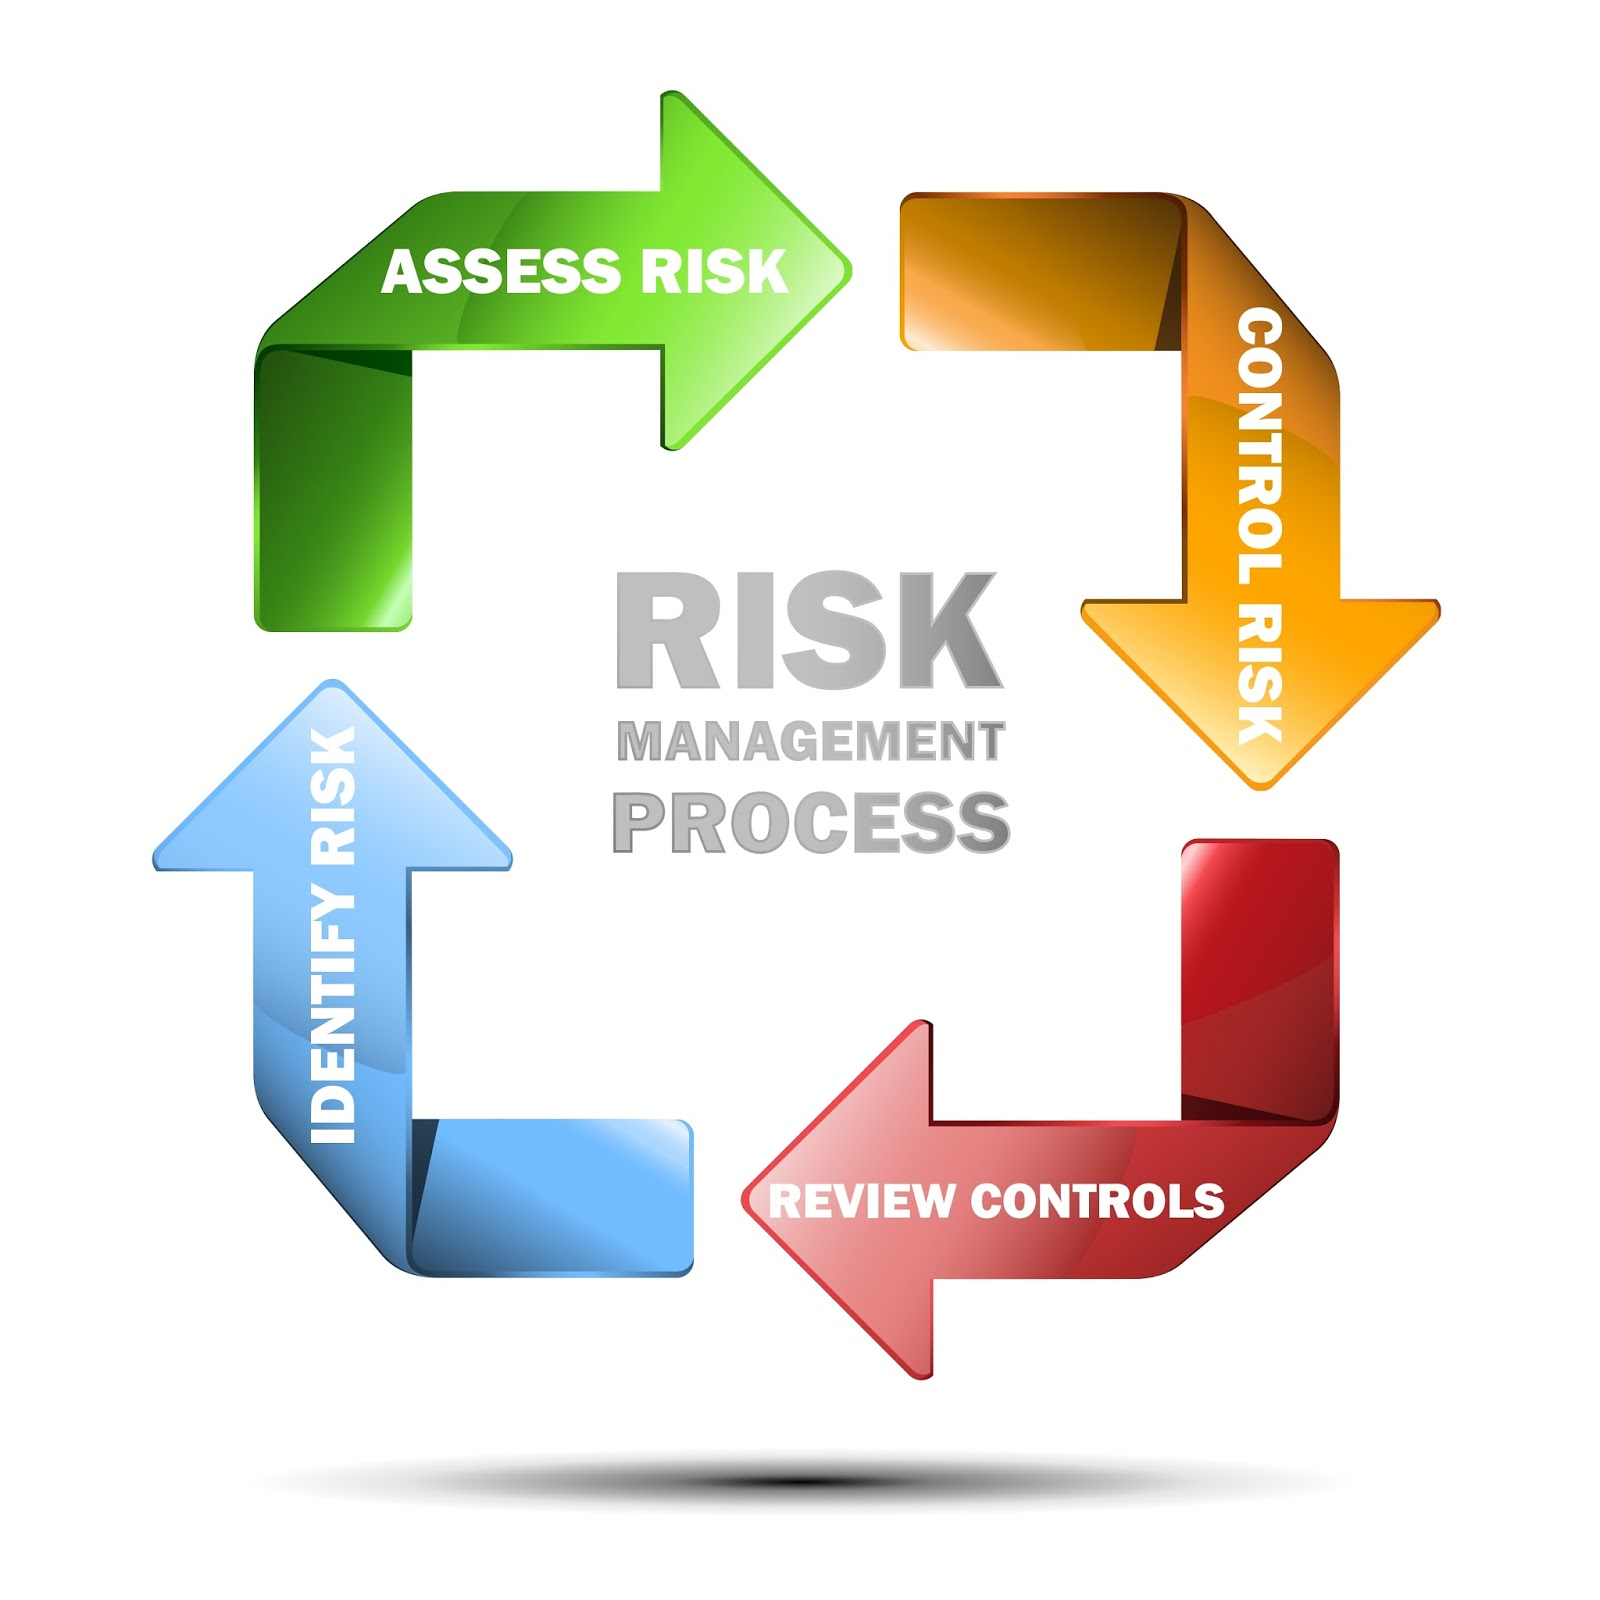
\includegraphics[width=0.3\textwidth]{risk-management-process.jpg}
    \caption{Risk Management Process}
\end{figure}

\subsection{Security Audit}

\begin{itemize}
    \item Self assessment
    \item Externe audit
    \begin{itemize}
        \item Penetration test 
        \item Bv: Red teaming
        \item Red vs Blue: 2 teams
        \item Blue team verdedigt, Red team valt aan op een realistische manier
        \item Blue team weet niet per se dat er zal aangevallen worden
    \end{itemize} 
\end{itemize}

\subsubsection{Self assessment}

\begin{itemize}
    \item Incident response plan
    \item Review van de procedures
    \item Interne opleiding/informatie
    \item Controle van back-up en recovery procedures
\end{itemize}

\subsubsection{Externe audit}

\begin{itemize}
    \item Pentest (penetration test)
    \item Red-teaming (vs blue team)
    \item Gebruik van offensieve technieken
    \item Identificeert zwakheden
\end{itemize}


\subsection{Pentesting}

\begin{itemize}
    \item Black box testing 
    \item White box testing
    \item Grey box testing = combinatie van de twee. Als de Blackbox test niets opleverd kan je vragen voor bvb credentials van een user account, om dan daarmee verder te black box testen.
\end{itemize}

\begin{figure}[H]
    \centering
    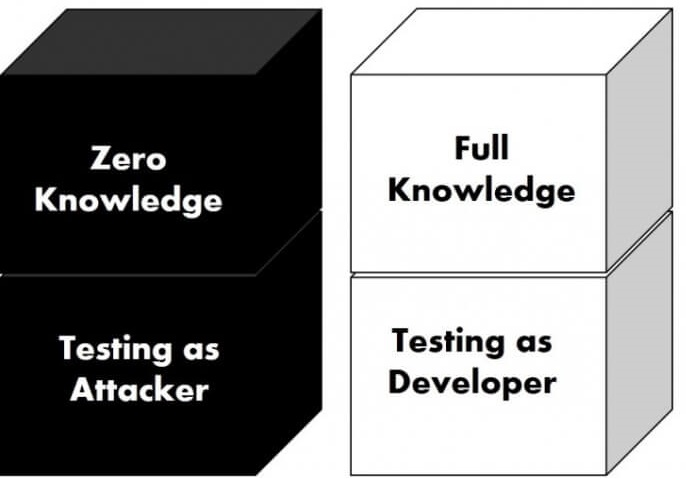
\includegraphics[width=0.4\textwidth]{pentesting.jpg}
    \caption{Black-box vs White-box testing}
\end{figure}

\subsubsection{Scope van een pentest}

\begin{itemize}
    \item Scope defini"eren: wat mag/kan getest worden
    \item Minimaliseren van bedrijfsimpact
    \item Behouden van de relevantie van de test
    \item Negatieve impact is niet uit te sluiten
    \item Opletten met derde partijen
\end{itemize}

\subsubsection{Resultaat van een pentest}

\begin{itemize}
    \item $\Rightarrow$ Pentest report
    \item Lange lijst (potenti"ele) kwetsbaarheden
    \item Is geen `score' of `certificaat'
    \item Duidelijk resultaat:
    \begin{itemize}
        \item Transparant
        \item Prioriteiten
        \item Aanbevelingen
    \end{itemize}
\end{itemize}

\subsection{Tegenmaatregelen}

= Mitigation

\begin{itemize}
    \item Corporate policy - Training - Awareness
    \item Coding practices
    \item Testing (pentesting)
    \item Vulnerability management
    \item Backup
    \item Disaster recovery plan
    \item Fysieke security
    \item Firewall / IDS / IPS
\end{itemize}

\subsection{Tips}

\begin{itemize}
    \item Security is geen taak maar een proces
    \item Security is nooit `af' maar in constante flux
    \item Informeer gebruikers (awareness) (herhaaldelijk)
    \item Ga voor de `quick wins'
    \item Elimineer `low-hanging fruit'
    \item Update software, infrastructuur en tools
    \item Maak een corporate policy
    \item Maak een disaster recover plan
    \item Zorg voor een correcte back-up
\end{itemize}

\section{IoT Security}

\begin{itemize}
    \item Securty vaak afwezig of slecht geimplementeerd
    \item Privacy?
    \item Cloud interface / versleuteling communicatie
    \item Firmware vaak niet beschikbaar of worden niet geupdatet
\end{itemize}

\subsection{Industrial security}

\begin{itemize}
    \item Stuxnet 
    \begin{itemize}
        \item = worm in Siemens-apperatuur
        \item Gebouwd om PLC's te infecteren met als doel een defect te veroorzaken in nucleaire installaties
        \item \url{https://nl.wikipedia.org/wiki/Stuxnet}
    \end{itemize}
    \item Oorzaak: Andere prioriteiten: CIA <> AIC
    \item Langere levensduur van systemen
    \item Moeilijker patchmanagement (conformiteit)
    \item SCADA interface op ICT netwerk voor ERP
\end{itemize}

\subsection{Industrial control systems (ICS)}

\begin{itemize}
    \item Robots
    \item Sensoren
    \item Productiemachines
    \item \bold{Securityprobleem:} men wil alles linken met elkaar en met het internet
\end{itemize}

\begin{figure}[H]
    \centering
    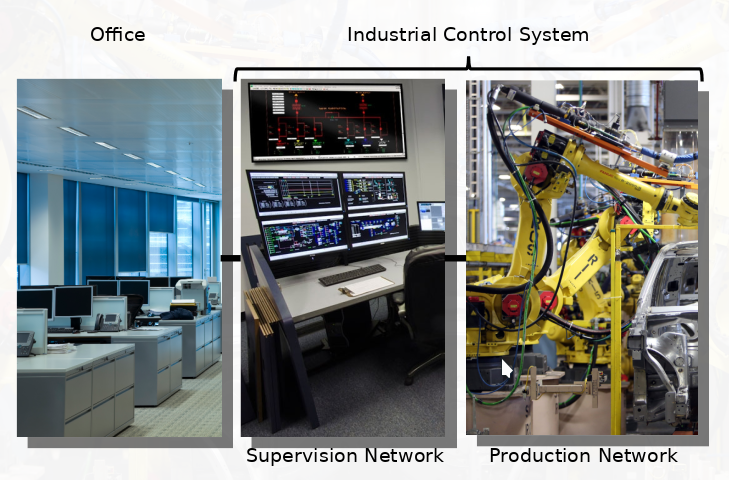
\includegraphics[width=0.5\textwidth]{iot-industrial-control-systems.png}
    \caption{Industrial control system (ICS)}
\end{figure}

\begin{figure}[H]
    \centering
    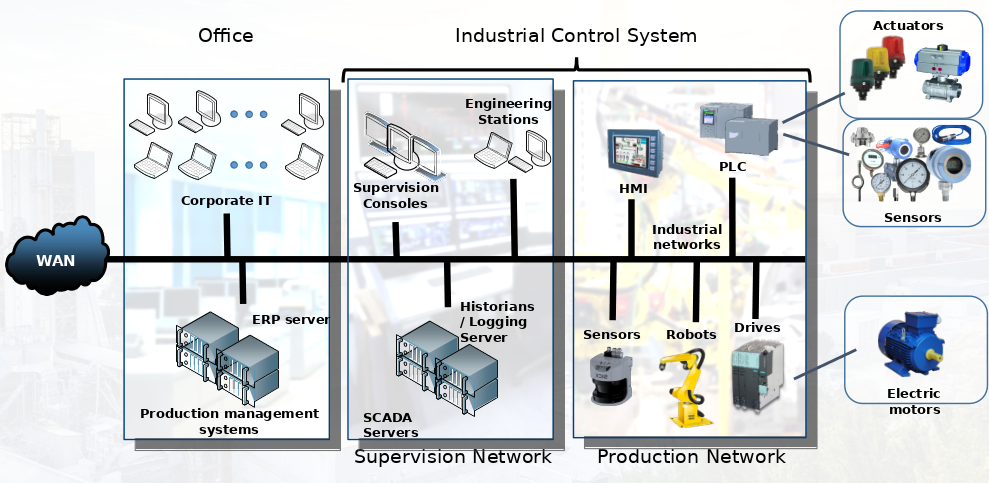
\includegraphics[width=0.5\textwidth]{iot-ics2.png}
    \caption{ICS schema}
\end{figure}

\subsubsection{In welke sectoren?}

Overal:

\begin{itemize}
    \item Kernenergie
    \item Olie \& gas
    \item Transport
    \item Water
    \item Pharmabedrijfen
    \item Groene energie
    \item \dots
\end{itemize}

\subsubsection{Protocollen}

\begin{figure}[H]
    \centering
    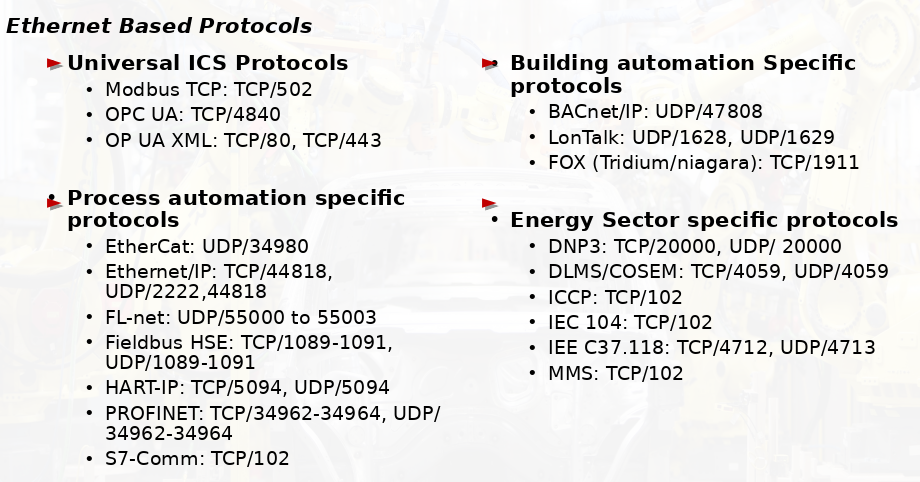
\includegraphics[width=0.5\textwidth]{iot-ics-protocollen.png}
    \caption{Industri"ele communicatie}
\end{figure}

\begin{itemize}
    \item Deze protocollen zijn niet echt ontwikkeld met veiligheid in het achterhoofd
    \item Alleen voor basisfunctionaliteit op meestal oude systemen
    \item Potenti"ele problemen (bv Shodan)
\end{itemize}

\section{Encryptie}

\begin{itemize}
    \item Gaat over:
    \begin{itemize}
        \item Geheimhouding
        \item Authenticatie
        \item Integriteit behouden
    \end{itemize}
    \item Helpt niet met beschikbaarheid (vaak het omgekeerde effect)
    \item Nonrepudation (=onweerlegbaarheid)
    \begin{itemize}
        \item "In authenticiteit, een dienst die zorgt voor het bewijs van de integriteit en oorsprong van de data, beide in een onvergetelijke relatie, welke geverifieerd kan worden door elke derde partij op elk moment"
        \item \url{https://nl.wikipedia.org/wiki/Onweerlegbaarheid#Crypto-technische\_betekenis}
    \end{itemize}
\end{itemize}

\subsection{Traditionele cryptografie}

\begin{itemize}
    \item Substitutie
    \item Transpositie
    \item One-time pad
\end{itemize}

\bold{Voorbeeld}: ROT-13: Schuif elke letter in een zin 13 plaatsen op in het alfabet:

`Een leesbare zin' $\Rightarrow$ `Rra yrrfoner mva'

\subsection{Symmetrische encryptie}

\begin{itemize}
    \item Alleen Geheimhouding
    \item \bold{Geen} authenticatie
    \item Eenvoudig
    \item Snel (performant)
\end{itemize}

\subsubsection{Triple DES}

\begin{itemize}
    \item Met 2 of 3 sleutels
    \item Verhoogde veiligheid
    \item Kan in hardware
\end{itemize}

\subsubsection{Voorbeelden}

\begin{itemize}
    \item DES
    \begin{itemize}
        \item Block-cipher van 64 bit
        \item 16 encryptiecycli met telkens andere subkey
        \item Bitlengte van de sleutel is bepalend, 56bit is tegenwoordig te laag
    \end{itemize}
    \item AES
    \begin{itemize}
        \item = Rijndael (originele naam)
        \item Advanced Encryption Standard
        \item Veiliger dan DES
    \end{itemize}
    \item IDEA
    \item CAST-128
    \item Blowfish (variabele sleutellengte)
\end{itemize}

\subsection{Assymetrische encryptie}

\begin{itemize}
    \item Public key encryptie, bv: \bold{RSA}, \bold{ECC}
    \item Geheimhouding
    \item Authenticatie
    \item Werkt met sleutel\bold{paren}
    \begin{itemize}
        \item Private sleutel (=geef je aan niemand)
        \item Publieke sleutel (= geef je aan iedereen)
    \end{itemize}
    \item Zeer berekeningsintensief
    \item Het is niet mogelijk om de private sleutel te berekenen uit de publieke sleutel
\end{itemize}

\subsection{Hashing}

= een bepaalde string van variabele lengte omzetten in iets met vaste lengte en vast format. 

\subsubsection{Eigenschappen}

\begin{itemize}
    \item Variabele inputlengte
    \item Vaste outputlengte
    \item Kleine inputvariatie resulteert in grote outputvariatie
    \item Niet reversibel
\end{itemize}

\subsubsection{Voorbeelden}

\begin{itemize}
    \item MD5
    \begin{itemize}
        \item MD5 is gekraakt: het is mogelijk om expres dezelfde hash te genereren uit een verschillende input via het MD5 algoritme.
        \item Daarom niet (meer) betrouwbaar
    \end{itemize}
    \item SHA2
    \item \dots
\end{itemize}

\subsection{Diffie-Hellman exchange}

\begin{itemize}
    \item Uitwisselen van een shared secret (key)
\end{itemize}

\begin{figure}[H]
    \centering
    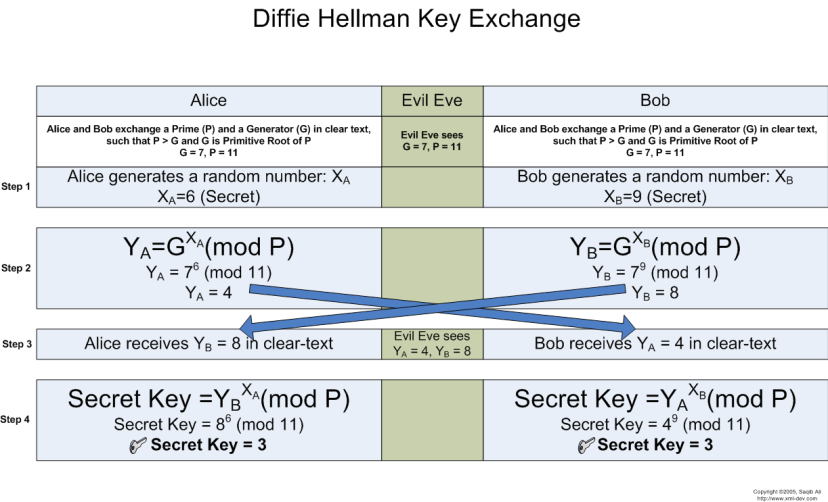
\includegraphics[width=0.8\textwidth]{diffie-hellman.png}
    \caption{}
\end{figure}

\subsection{Crypto algoritmes}

\subsubsection{Schneier's Law}

Anyone, from the most clueless amateur to the best cryptographer, 
can create an algorithm that he himself can't break. 
It's not even hard. What is hard is creating an algorithm that no one else can break, 
even after years of analysis. 
And the only way to prove that is to subject the algorithm to years of analysis by the best cryptographers around.


\begin{itemize}
    \item \bold{Laat het ontwerpen van crypto over aan professionals}
    \item \url{http://www.moserware.com/2009/09/stick-figure-guide-to-advanced.html}
\end{itemize}

\subsection{Veilige websites}

\begin{itemize}
    \item HTTPS ipv HTTP voor `velige' verbindingen
    \item Kwaadwillige sites kunnen ook HTTPS gebruiken
    \item SSL betekent enkel dat gegevens niet kunnen worden afgeluisterd
\end{itemize}

\subsubsection{Praktisch gebruik}

\begin{itemize}
    \item SSL certificaten
    \item E-mail versleutelen
    \item E-mail afzender identificatie
    \item Websites
    \item API's
    \item \dots
\end{itemize}

\subsection{Belangrijke tips}

\begin{itemize}
    \item Gebruik steeds een correct algoritme voor de toepassing
    \item Checksum != hashing
    \item CRC (cyclic redundancy check) is OK voor foutcontrole, niet voor authenticatie
    \begin{itemize}
        \item Voorbeeld: check op rekeningnummers / creditkaarten
    \end{itemize} 
\end{itemize}

\subsection{PKI}

= Public Key Infrastructure

\begin{itemize}
    \item Assymtrische encryptie: met public en private key
\end{itemize}

\subsubsection{Doel}

Het versturen van een geheim bericht over een onveilig medium.

\subsubsection{Stappenplan om een tekst te versleutelen}

\begin{enumerate}
    \item Alice en Bob willen communiceren
    \item Alice en Bob maken elk een sleutelpaar (private en public)
    \item De publieke sleutel van Alice sturen we naar Bob
    \item De publieke sleutel van Bob sturen we naar Alice
    \item Alice wil een tekst veilig doorsturen
    \item Alice maakt een hash van de tekst. De tekst wordt versleuteld met behulp van haar private sleutel
    \item Bob decodeert de sleutel met behulp van de publieke sleutel van Alice
\end{enumerate}

\subsubsection{Wat als er een Man In The Middle is?}

Man in the middle = Eve

\begin{enumerate}
    \item Eve stuurt een publieke sleutel naar Alice en zegt dat die van Bob is
    \item Eve stuurt een publieke sleutel naar Bob en zegt dat die van Alice is
    \item Eve kan berichten sturen in naam van Alice en Bob
\end{enumerate}

\subsubsection{Hoe een publieke sleutel veilig versturen?}

Gebruikmaken van een CA (=Certificate Authority)

\begin{itemize}
    \item Gecentraliseerde authoriteit
    \item Zowel Alice als Bob aanvaarden de authoriteit van de CA
    \item De CA genereert een sleutelpaar (publiek en privaat)
    \item Iedereen kent de publieke sleutel (inbouwen in alle computers, zit in de Certificate Store van Windows of wordt via browsers meegegeven)
    \item Alice stuurt haar eigen publieke sleutel deze keer niet naar Bob, maar naar de CA. Bob doet hetzelfde
    \item De CA zal de public key van Alice versleutelen met zijn eigen private key. Alice krijgt deze digitale handtekening om te bevestigen op haar publieke sleutel.
    \item Alice heeft nu een publieke sleutel die is voorzien van een digitale handtekening van de CA
    \item Nu zal Alice haar publieke sleutel gehandtekend naar Bob sturen
    \item Communicatie kan nu veilig verlopen.
\end{itemize}

Er zijn wel nog 2 problemen:

\begin{enumerate}
    \item De private key van de CA mag NOOIT gekend worden
    \item Er bestaan ook Fake CA's (al gebeurd bij Dell)
\end{enumerate}

\section{DNS}

Wordt gebruikt om een FQDN (Fully Qualified Domain Name) om te zetten naar een IP-adres

\begin{figure}[H]
    \centering
    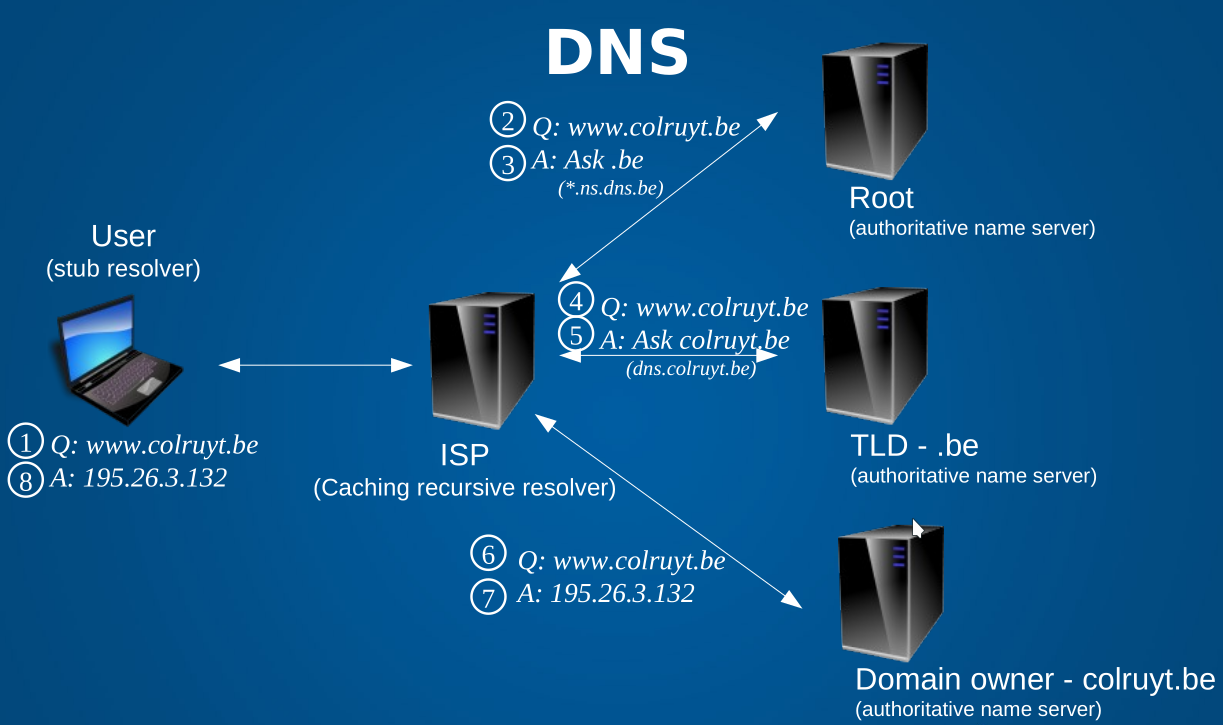
\includegraphics[width=0.7\textwidth]{dns.png}
    \caption{Werking DNS}
\end{figure}


\subsection{Potenti"ele problemen met DNS}

\begin{itemize}
    \item Een van de oudste protocollen op het internet
    \item Gemaakt in de tijd waar hosts gekend en vertrouwd waren
    \item Het design van DNS is onveilig, security was geen vereiste
\end{itemize}

\subsection{2 Attack vectors}

\begin{enumerate}
    \item Channel
    \begin{itemize}
        \item = De verbinding tussen de servers, de clients en de resolvers
    \end{itemize}
    \item Data (in caches)
    \begin{itemize}
        \item Wat er wordt verstuurd
        \item Cache poisoning, Man-in-the-middle
        \item Wijziging van data (ip adressen van betrouwbare sites vervangen door eigen ip adres)
        \item Kaminsky attack
    \end{itemize}
\end{enumerate}

\subsection{Kaminsky Attack}

\begin{itemize}
    \item Je zorgt dat de resolver geen gecachte informatie heeft over een bepaald domain
    \item Je vraagt informatie over dat domein
    \item Je geeft direct een antwoord met je eigen informatie
    \item Zo zorg je ervoor dat elke client die informatie vraagt de verkeerde informatie krijgt
\end{itemize}

\subsection{DNSSEC}

\begin{itemize}
    \item = DNS Security Extensions
    \item Gemaakt om het DNS protocol te voorzien van een digitale handtekening
    \item Beveiligen tegen bovenstaande attack vectors
    \item Met publieke en private sleutels
    \item Omdat de publieke sleutel zichtbaar is voor iedereen, is die na heel lange tijd kraakbaar $\Rightarrow$ sleutel moet na bepaalde tijd verlopen
    \item Daarom worden 2 types sleutels gebruikt:
    \begin{enumerate}
        \item Zone Signing Key (ZSK): korter, kwetsbaarder, moet sneller vervangen worden
        \item Key Signing Key (KSK), wordt gebruikt om de sleutels zelf te authenticeren, cryptografisch sterker
    \end{enumerate}
\end{itemize}

\begin{figure}[H]
    \centering
    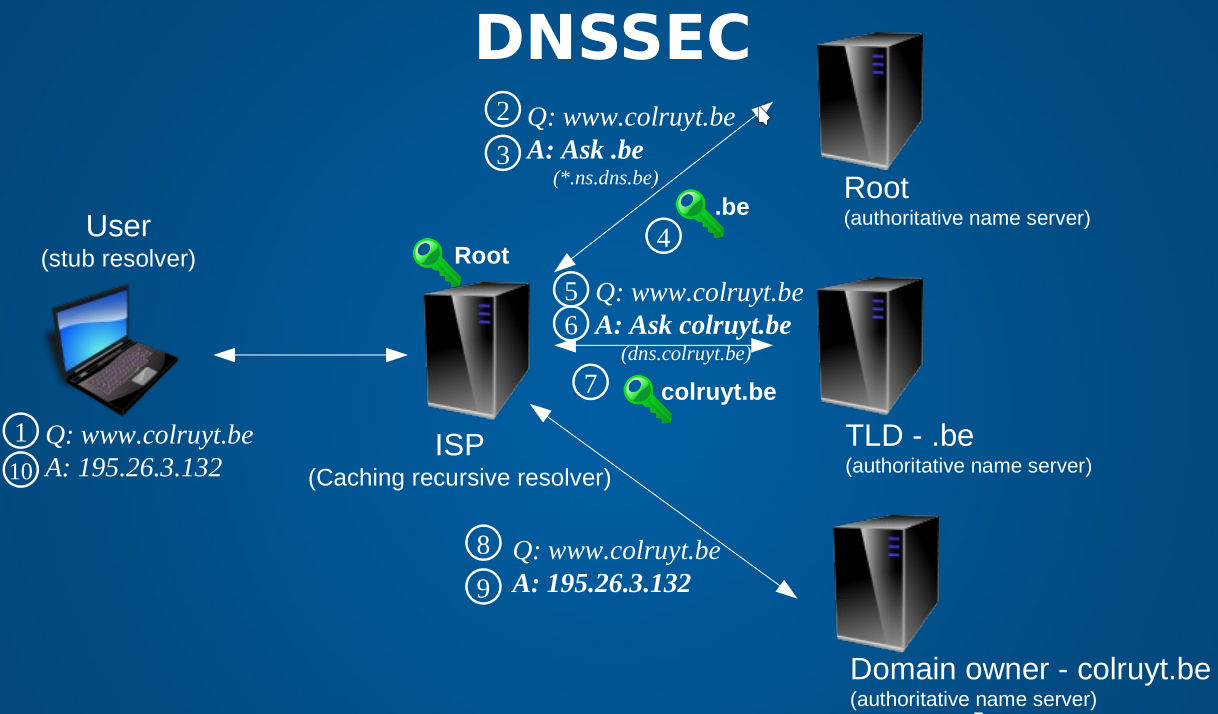
\includegraphics[width=0.7\textwidth]{dnssec.png}
    \caption{DNSSEC}
\end{figure}

\subsubsection{Algoritmes}

\begin{itemize}
    \item Vroeger: MD5
    \item Nu: RSA
\end{itemize}

\subsubsection{NSEC records}

\bold{Probleem:} Die gepubliceerde informatie wordt enkel gecertificeerd voor records die al bestaan. 
Er is niet dat men tegenhoudt om een nieuw subdomain te maken voor een bestaand domein om daar een soort Kaminsky attack op toe te passen.
Manier nodig om te zeggen of een subdomain bestaat of niet.

\bold{Oplossing:} NSEC records

\begin{itemize}
    \item Record die subdomein bijhoudt
    \item Elke record verwijst naar de volgende entry
    \item De records staan in alfabetische volgorde
    \item Problemen:
    \begin{itemize}
        \item Meer belasting op systeem
        \item Alle records zijn enumereerbaar
        \item = \bold{Zone walking}
    \end{itemize}
\end{itemize}

\begin{figure}[H]
    \centering
    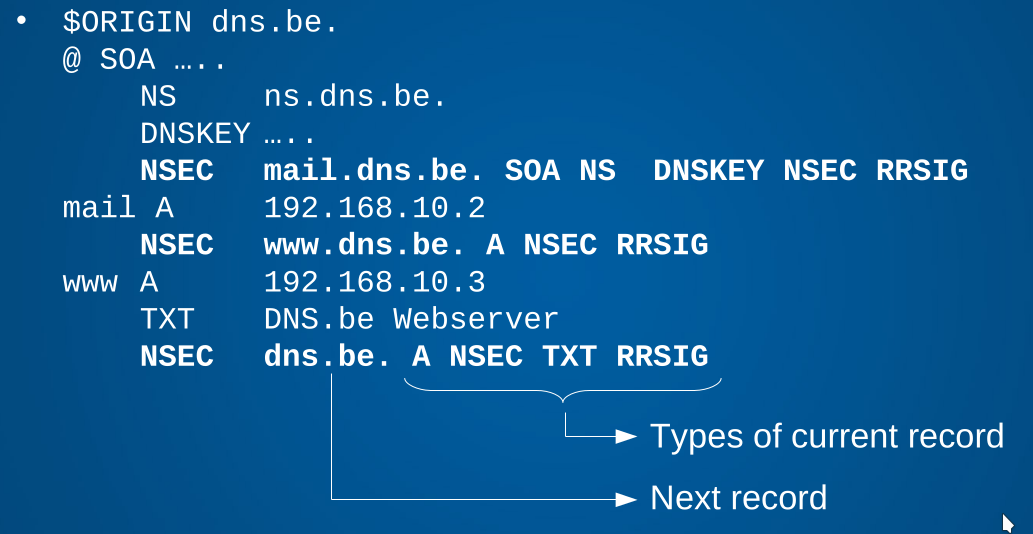
\includegraphics[width=0.5\textwidth]{nsec.png}
    \caption{Het NS-record bestaat altijd $\Rightarrow$ de rest is enumereerbaar via de NSEC records}
\end{figure}

Dit is dus een zeer groot probleem

\subsubsection{NSEC3}

\begin{itemize}
    \item NSEC records worden gehashed
    \item Nog altijd alfabetisch
\end{itemize}

\section{Exploits}

= stukjes code om een bepaalde kwetsbaarheid uit te buiten

\begin{itemize}
    \item Reversing 
    \item Decompilers
    \item Debuggers
\end{itemize}

\subsection{Reverse engineering}

\begin{itemize}
    \item Let op met IL-talen (Intermediate Language) = Java/.NET/\dots, alles dat reflection ondersteund
    \item Obfuscatie is mogelijk, maar gebeurt meestal volgens vaste methodes, dus deobfuscatie kan gebeuren 
\end{itemize}

\subsection{Fuzzing}

\begin{itemize}
    \item Random dingen proberen tot iets onverwachts gebeurt
    \item Dit kan je dan onderzoeken (in een debugger) en uitbuiten (met bv een buffer overflow of een use-after-free)
\end{itemize}

\subsection{Shellcode}

\begin{itemize}
    \item = ASCII-gecodeerde uitvoerbare code
    \item Shellcode in memory proberen te krijgen om te exploiten
    \item Om bijvoorbeeld te springen over een if-statement
    \item Let op voor Endianness: Little Endian != Big Endian. Heel veel protocollen keren de volgorde van de bytes om.
\end{itemize}


\section{Examenvragen}

\begin{itemize}
    \item Wat is een buffer overflow?
    \item Hoe beveilig je tegen een buffer overflow?
    \item Geef een paar voorbeelden van vulnerability scanners 
    \begin{itemize}
        \item (penVas, Nessus, Nikto, wpscan, joomscan \dots
    \end{itemize}
    \item Types encryptie + voorbeelden
    \item Wat is AES? Wat is RSA? Nadelen?
    \item Wat is het verschil tussen checksums en hashing?
    \item Het Diffie-Hellman-protocol wordt gebruikt om...
    \begin{itemize}
        \item Een shared secret uit te wisselen 
    \end{itemize}
    \item Volgens de GDPR moet je een nette werkplaats hebben, waar of niet waar?
    \begin{itemize}
        \item Waar: Clean desk policy
    \end{itemize}
\end{itemize}

\end{document}